\documentclass[12pt,a4paper]{article}
\usepackage[utf8]{inputenc}
%\usepackage[left=2.00cm,right=2.00cm,top=2.00cm,bottom=2.00cm]{geometry}
\usepackage{transparent}
\usepackage{amsmath}                                 % AMS Math Package
\usepackage{amssymb}                                 % Math symbols such as \mathbb
\usepackage{graphicx}                                % Allows for eps images
\usepackage[dvips,margin=1in,bottom=1in]{geometry}
\usepackage{tensor}
\usepackage{tcolorbox}
\usepackage[explicit,compact]{titlesec}
\usepackage{csquotes}
\usepackage{amsthm}
\usepackage{mathtools}
\usepackage{booktabs}

\titlespacing\section{0pt}{12pt plus 4pt minus 2pt}{0pt plus 2pt minus 2pt}
\titlespacing\subsection{0pt}{12pt plus 4pt minus 2pt}{0pt plus 2pt minus 2pt}
\titlespacing\subsubsection{0pt}{12pt plus 4pt minus 2pt}{0pt plus 2pt minus 2pt}

%\titleformat{\part}[hang]{\Huge\bfseries\sffamily}{}{0pt}{
%\begin{tcolorbox}[width=3cm,height=1.5cm,colback=black!75!white,colframe=black!75!white,center title,fonttitle=\bfseries\normalsize,title=PART,text fill]
%	\centering
%	{\color{white}\thepart}
%\end{tcolorbox}
%}

\titleformat{\part}[display]{\Huge\bfseries}{
	\vspace{-1.2cm}
	\begin{minipage}[t]{0.8\columnwidth}
		#1
	\end{minipage}
	\hfill
	\begin{minipage}[t]{0.2\columnwidth}
		\begin{tcolorbox}[width=3cm,height=1.5cm,colback=black!75!white,colframe=black!75!white,center title,fonttitle=\bfseries\normalsize,title=PART,text fill,flush right]
			\begin{center}
				{\color{white}\thepart}
			\end{center}
		\end{tcolorbox}
	\end{minipage}
	\vspace{-2cm}
	}{0pt}{}

\titlespacing{\part}{0pt}{0pt minus 2pt}{-\parskip}


% Sets margins and page size

\usepackage{amsmath, esint,mathrsfs}
\def\doubleunderline#1{\underline{\underline{#1}}}
\renewcommand{\labelenumi}{(\alph{enumi})}                % Use letters for enumerate

\usepackage{enumerate}
\usepackage{caption}
\usepackage[]{algorithm2e}

\usepackage{listings}
\usepackage{xcolor}



\definecolor{codegreen}{rgb}{0,0.6,0}
\definecolor{codegray}{rgb}{0.5,0.5,0.5}
\definecolor{codepurple}{rgb}{0.58,0,0.82}
\definecolor{backcolour}{rgb}{0.97,0.97,0.97}

\lstdefinestyle{mystyle}{
	language=Python,
	backgroundcolor=\color{backcolour},   
	commentstyle=\color{codegreen},
	keywordstyle=\color{magenta},
	numberstyle=\tiny\color{codegray},
	stringstyle=\color{codepurple},
	basicstyle=\ttfamily\footnotesize,
	breakatwhitespace=false,         
	breaklines=true,                 
	captionpos=b,                    
	keepspaces=true,                 
	numbers=left,                    
	numbersep=5pt,                  
	showspaces=false,                
	showstringspaces=false,
	showtabs=false,                  
	tabsize=2
}

\lstset{style=mystyle}

\newcommand{\gv}[1]{\ensuremath{\mbox{\boldmath$ #1 $}}} 
\newcommand{\uv}[1]{\ensuremath{\mathbf{\hat{#1}}}}       % enhetsvektor
\newcommand{\abs}[1]{\left| #1 \right|}                   % abslouttverdi
\newcommand{\avg}[1]{\left< #1 \right>}                   % gjennomsnitt

\newcommand{\der}[2]{\frac{\text{d} #1}{\text{d} #2}}     % derivert
\newcommand{\dd}[2]{\frac{\text{d}^2 #1}{\text{d}#2^2}}   % dobbelderivert
\newcommand{\pd}[2]{\frac{\partial #1}{\partial #2}}      % partiellderiverte
\newcommand{\pdd}[2]{\frac{\partial^2 #1}{\partial #2^2}} % doble partiellderiverte

% Kvantemekanikk:

\newcommand{\ket}[1]{\left| #1 \right>}                    % for Dirac kets
\newcommand{\bra}[1]{\left< #1 \right|}                    % for Dirac bras
\newcommand{\braket}[2]{\left< #1 \vphantom{#2} \right|
	\left. #2 \vphantom{#1} \right>}                       % for Dirac brackets
\newcommand{\matrixel}[3]{\left< #1 \vphantom{#2#3} \right|
	#2 \left| #3 \vphantom{#1#2} \right>}                  % for Dirac matrix elements

% Vektoranalyse

\newcommand{\grad}[1]{\gv{\nabla} #1}                      % gradient
\let\divsymb=\div                                          % nytt navn til div
\renewcommand{\div}[1]{\gv{\nabla} \cdot \v{#1}}           % divergens
\newcommand{\curl}[1]{\gv{\nabla} \times \v{#1}}           % curl


% div macros

\newcommand{\iu}{\textup{i}} % imaginary unit
\newcommand{\e}{\textup{e}} % exponent
\newcommand{\intd}[1]{\int\text{d}#1}

% document layout

\setlength{\parindent}{0em}
\setlength{\parskip}{1em}
\setlength{\parindent}{0pt}

\usepackage{nameref}
\usepackage{fancyhdr}
\usepackage{csvsimple}

\author{Sondre Duna Lundemo}

\newcommand\bluetextit[1]{\textcolor{blue}{\textit{\sffamily#1}}}
\newcommand\bluetextbf[1]{\textcolor{blue}{\textbf{\sffamily#1}}}

\pagestyle{fancy}
\renewcommand{\headrulewidth}{0.5pt}
\fancyhf{}
\rhead{\textit{\fontfamily{cmr}\selectfont Cand. $10037$}}
\lhead{\small \textsc{\rightmark}}
\cfoot{\textemdash \, \thepage \, \textemdash}

%\titleformat*{\section}{\bfseries \Large #1 }
%\titleformat*{\subsection}{\bfseries\large #1}
%\titleformat*{\subsubsection}{\bfseries \normalsize #1 }

\fancypagestyle{titlepage}{
	\fancyhf{}
	\fancyfootoffset{-4cm}
	\renewcommand{\headrulewidth}{0pt}
	\renewcommand\footrulewidth{0.5pt}
}

% theoremstyles

\theoremstyle{plain}
\newtheorem{thm}{Theorem}
\newtheorem{axiom}{Axiom}

\theoremstyle{definition}

\newtheorem{definition}{Definition}
\newtheorem{lemma}{Lemma}
\newtheorem{cor}{Corollary}
\newtheorem{prop}{Proposition}

\theoremstyle{remark}

\newtheorem{remark}{Remark}
\newtheorem{notation}{Notation}

\usepackage{enumitem}

\def\be{\begin{equation}}
\def\ee{\end{equation}}

\def\bse{\begin{equation*}}
\def\ese{\end{equation*}}

\def\bt{\begin{thm}}
\def\et{\end{thm}}

\def\bl{\begin{lemma}}
\def\el{\end{lemma}}

\def\bc{\begin{cor}}
\def\ec{\end{cor}}

\def\br{\begin{remark}}
\def\er{\end{remark}}

\def\bal{\begin{align}}
	\def\eal{\end{align}}
	
\def\bd{\begin{definition}}
	\def\ed{\end{definition}}

\def\bit{\begin{itemize}}
	\def\eit{\end{itemize}}

\def\bt{\begin{thm}}
	\def\et{\end{thm}}

\let\vaccent=\v % rename builtin command \v{} to \vaccent{}
\renewcommand{\v}[1]{\ensuremath{\mathbf{#1}}} % vektor

%miscellaneous shortcuts

\providecommand{\AA}{\mathbb{A}}
\providecommand{\BB}{\mathbb{B}}
\providecommand{\CC}{\mathbb{C}}
\providecommand{\DD}{\mathbb{D}}
\providecommand{\EE}{\mathbb{E}}
\providecommand{\FF}{\mathbb{F}}
\providecommand{\GG}{\mathbb{G}}
\providecommand{\HH}{\mathbb{H}}
\providecommand{\II}{\mathbb{I}}
\providecommand{\JJ}{\mathbb{J}}
\providecommand{\KK}{\mathbb{K}}
\providecommand{\LL}{\mathbb{L}}
\providecommand{\MM}{\mathbb{M}}
\providecommand{\NN}{\mathbb{N}}
\providecommand{\OO}{\mathbb{O}}
\providecommand{\PP}{\mathbb{P}}
\providecommand{\QQ}{\mathbb{Q}}
\providecommand{\RR}{\mathbb{R}}
\providecommand{\SS}{\mathbb{S}}
\providecommand{\TT}{\mathbb{T}}
\providecommand{\UU}{\mathbb{U}}
\providecommand{\VV}{\mathbb{V}}
\providecommand{\WW}{\mathbb{W}}
\providecommand{\XX}{\mathbb{X}}
\providecommand{\YY}{\mathbb{Y}}
\providecommand{\ZZ}{\mathbb{Z}}

\providecommand{\A}{\mathcal{A}}
\providecommand{\B}{\mathcal{B}}
\providecommand{\C}{\mathcal{C}}
\providecommand{\D}{\mathcal{D}}
\providecommand{\E}{\mathcal{E}}
\providecommand{\F}{\mathcal{F}}
\providecommand{\G}{\mathcal{G}}
\providecommand{\H}{\mathcal{H}}
\providecommand{\I}{\mathcal{I}}
\providecommand{\J}{\mathcal{J}}
\providecommand{\K}{\mathcal{K}}
\providecommand{\L}{\mathcal{L}}
\providecommand{\M}{\mathcal{M}}
\providecommand{\N}{\mathcal{N}}
\providecommand{\CO}{\mathcal{O}}
\providecommand{\P}{\mathcal{P}}
\providecommand{\Q}{\mathcal{Q}}
\providecommand{\R}{\mathcal{R}}
\providecommand{\S}{\mathcal{S}}
\providecommand{\T}{\mathcal{T}}
\providecommand{\U}{\mathcal{U}}
\providecommand{\V}{\mathcal{V}}
\providecommand{\W}{\mathcal{W}}
\providecommand{\X}{\mathcal{X}}
\providecommand{\Y}{\mathcal{Y}}
\providecommand{\Z}{\mathcal{Z}}

\usepackage{hyperref}
\hypersetup{colorlinks=true,linkcolor=blue}

\begin{document}
	
\begin{titlepage}
	\begin{center}
	\setlength{\parskip}{0em}
	\thispagestyle{titlepage}
	
	\centering{
		\Huge{\textbf{ Exam: Epidemic modelling }}
	}

	\vspace{4mm}
	
	\large{\textbf{Candidate nr. $10037$ }}
	
	\normalsize{Department of Physics, Norwegian University of Science and Technology, Trondheim Norway \\
	TFY4235 - Computational physics
	}

	(\textit{Last updated on \today})
	\end{center}

	\setlength{\parindent}{2em}
		
		\begin{abstract}
		We study various models for the time evolution of epidemics, including deterministic and stochastic SIR-models, stochastic SEIIaR models and stochastic SEIIaR commuter models. These are applied to a variety of systems, starting small and towards the end applied on a system representing the working population of Norway. 
		\end{abstract}
	\begin{figure}[htb]
		% front fig ? 
	\end{figure}
	

\end{titlepage}

\newpage
\setlength{\parskip}{0em}
\tableofcontents
\setlength{\parskip}{1em}
\newpage

\part{Introduction}

The topic of this project is epidemic modelling. A short introduction to the models under consideration are given in this introduction, mostly for introducing notation and presenting some choices in the implementation. For a more detailed introduction, consult the problem sheet \cite{sheet}.

\subsection{The deterministic SIR model}
The SIR model describes the evolution of \textbf{S}usceptible, \textbf{I}nfected and \textbf{R}ecovered people in an epidemic. The model reads
\begin{subequations}\label{eq:SIR}
\begin{align}
	\der{S}{t} &= - \beta \frac{I S}{N}\\
	\der{I}{t} &= \beta \frac{IS }{N} - I/\tau \\
	\der{R}{t} &= I/\tau, 
\end{align}
\end{subequations}
where $\beta$ is the rate at which susceptible people encounter infected people, and become infected, and $\tau$ is the typical duration of the infection. To solve these equations numerically, we recast it to a system of ODE's by defining the vector $\mathbf{v} = [S,I,R]^T$, such that the equations in \ref{eq:SIR} simplify to
\begin{equation}\label{eq:sir_vect}
	\der{\mathbf{v}(t)}{t} = \frac{\mathrm{d}}{\mathrm{d}t} \begin{bmatrix}
		S(t) \\
		I(t) \\
		R(t)
	\end{bmatrix}
	= \begin{bmatrix}
		- \beta IS/N \\
		\beta  IS/N - I/\tau \\
		I/\tau
	\end{bmatrix} = \begin{bmatrix}
		-\beta v_1 v_2 /N \\
		\beta v_1 v_2 - v_2/\tau \\
		v_2 / \tau
	\end{bmatrix}= \mathbf{f}(t,\mathbf{v}).
\end{equation}

\subsection{The stochastic SIR model}\label{sec:stochsirtheory}

For the stochastic SIR model we have probabilities instead of rates. The probabilities for a susceptible person becoming infected, and an infected person recovering during a time $\Delta t$ are given by
\begin{subequations}\label{eq:Psir}
	\begin{align}
		P_{S\to I} &= 1- \exp{(-\Delta t \beta I /N)} \\
		P_{I\to R} &= 1- \exp{(-\Delta t /\tau)},
	\end{align}
\end{subequations}
respectively. The transition to next time step is then governed by 
\begin{subequations}\label{eq:sir_disc}
	\begin{align}
		S(t + \Delta t) &= S(t) - \Delta_{S\to I} \\
		I(t + \Delta t) &= I(t) + \Delta_{S\to I} - \Delta_{I\to R} \\
		R(t + \Delta t) &= R(t) + \Delta_{I \to R}, \\
	\end{align}
\end{subequations}
where the $\Delta$'s are drawn from binomial distributions:
\begin{subequations}
	\begin{align*}
		\Delta_{S\to I } &= \mathcal{B}(S,P_{S \to I}) \\
		\Delta_{I\to R } &= \mathcal{B}(I,P_{I \to R}).
	\end{align*}
\end{subequations}
To see the connection between this model and the deterministic one, suppose $\Delta t  \beta \ll 1$, and $\Delta t/\tau \ll 1$. In that case, the probabilities in equation \eqref{eq:Psir} are in the first approximation given by
\begin{subequations}
	\begin{align}
		P_{S\to I} &\simeq \Delta t \beta I/N \\
		P_{I\to R} &\simeq \Delta t/\tau. 
	\end{align}
\end{subequations}
In the limit where $n\to \infty$\footnote{More formally, $n\to \infty$ and $p\to 0$ in such a fashion that the product $np$ is finite. }, the binomial distribution with $n$ samples and probability $p$ converges to a Poisson distribution with $\lambda = np$ \cite{Wassermann}, i.e. 
\begin{subequations}
	\begin{align}
		\Delta_{S\to I} &\to \mathrm{Pois}(SI \Delta t \beta/N) \\
		\Delta_{I\to R} &\to \mathrm{Pois}(I \Delta t/\tau).
	\end{align}
\end{subequations}
We can find expressions for the $\Delta$'s if we assume them to attain the mean value of the Poisson distributions, namely $\lambda$:
\begin{subequations}
	\begin{align}
		\Delta_{S\to I} &\simeq SI \Delta t \beta/N  \\
		\Delta_{I\to R} &\simeq I \Delta t/\tau.
	\end{align}
\end{subequations}
Hence, the discrete transition equations \eqref{eq:sir_disc} are then  
\begin{subequations}
	\begin{align}
		S(t + \Delta t) - S(t) &\simeq  - SI \Delta t \beta/N\\
		I(t + \Delta t) - I(t)&\simeq  + SI \Delta t \beta/N - I \Delta t/\tau \\
		R(t + \Delta t) -  R(t)&\simeq + I \Delta t/\tau, \\
	\end{align}
\end{subequations}
which yields the same equations as the deterministic ones in \eqref{eq:SIR}, by dividing all equations by $\Delta t$ and formally taking the limit $\Delta t \to 0$.

\subsection{The stochastic SEIIaR model}

For the stochastic SEIIaR model we follow essentially the same line of thought as for the stochastic SIR model, except that we include $E$ : exposed people, that cannot infect others, and $I_a$ : infected but asymptomatic people. The probabilities for the different transitions happening during an interval $\Delta t$ are
\begin{subequations}
	\begin{align}
		P_{S\to E} &= 1- \exp{\left(-\Delta t \beta \frac{r_s I + r_a I_a}{N}\right)} \\
		P_{E\to I} &=  f_s \times (1- \exp{(-\Delta t /\tau_E)}) \\
		P_{E\to I_a} &= f_a \times (1- \exp{(-\Delta t/\tau_E)}) \\
		P_{I\to R} &= 1- \exp{(-\Delta t /\tau_I)} \\
		P_{I_a\to R} &= 1- \exp{(-\Delta t/\tau_I)}, 
	\end{align}
\end{subequations}
with the different parameters $r_a,r_s,f_a,f_s,\tau_E,\tau_I$ given in \cite{sheet}. As before, 
\begin{subequations}
	\begin{align*}
		\Delta_{S\to E  } &= \mathcal{B}(S,P_{S \to E}) \\
		\Delta_{I\to R  } &= \mathcal{B}(I,P_{I \to R}) \\
		\Delta_{I_a\to R} &= \mathcal{B}(I_a,P_{I_a \to R}).
	\end{align*}
\end{subequations}
and 
\begin{equation}
	\Delta_{E \to I}, \Delta_{E \to I_a}, \Delta_{E \to E} = \mathcal{M}(E,(P_{E\to I},P_{E\to I_a}, (1- P_{E\to I} - P_{E\to I_a}))),
\end{equation}
where $\mathcal{M}$ denotes a multinomial distribution, as described in \cite{sheet}. The changes of the different variables during an interval $\Delta t$ are then given by
\begin{subequations}
	\begin{align}
		S(t + \Delta t) &= S(t) - \Delta_{S\to E} \\
		E(t + \Delta t) &= E(t) + \Delta_{S\to E} - \Delta_{E\to I} - \Delta_{E \to I_a} \\
		I(t + \Delta t) &= I(t) + \Delta_{E\to I} - \Delta_{I\to R} \\
		I_a(t + \Delta t) &= I_a(t) + \Delta_{E\to I_a} - \Delta_{I_a\to R} \\
		R(t + \Delta t) &= R(t) + \Delta_{I_a \to R} + \Delta_{I \to R}. \\
	\end{align}
\end{subequations}
To denote a state of the system, I will use $\mathbf{X} = [S,E,I,I_a,R]^T$. 

\vspace{2cm}

\part{Code overview}

The source code for this project is structured into separate files for each sub-problem, i.e. \lstinline|prob_2A.py|, \lstinline|prob_2B.py| etc. Additionally, there is a file for plotting for each sub-problem. I have also included a file called \lstinline|utils.py| which contains some useful utility functions used throughout the exercises. For problem $2$A I have used the same ODE-solver as the one I made for exercise $2$. This can be found in \lstinline|ode.py|.

\subsection{Remarks on performance}

In many parts I gained a lot of performance by compiling the code with \lstinline|numba|, as usual. 

My solution for solving the commuter model worked reasonably well in problem 2D, but when I reached problem 2E I found it to be \textit{very} memory consuming, as I store the number of people in each state for each group of people for each time step, which amounts to an array of size
$$
	\#\text{time steps}\times\#\text{towns} \times\#\text{towns} \times 5.
$$ 
For the population structure in problem 2Eb this yields an array of approximately $4.7$ GiB when using $1000$ time steps. To avoid these memory issues I modify the solver to only save the number of people in each state for each group of people for the current and previous time step. This allows for running short time steps without any memory issues, which, importantly,  makes it possible to run the $10$ simulations in parallel. 

From profiling the code used in problem 2Eb I found that the most time consuming part was the stepping function which draws random numbers for each entry in the matrix. I initially tried to draw these random numbers in a vectorised fashion, but found I it exceedingly hard to understand what the functions were doing when providing multidimensional inputs, and I started to get issues with people disappearing from the population. However, I found major improvements just by modifying the line where I step forward using the function \lstinline|SEIIaR_commuter_step()| to the following:
\begin{lstlisting}[language=Python]
if M[l,k] == 0:
    X[l,k,:] = X_[l,k,:]
else:
    X[l,k,:] = SEIIaR_commuter_step(X_[l,k,:],Pse[k],Pei,Peia,Pir,Piar)
\end{lstlisting} 

This is particularly useful in the case of problem 2Eb and c, as there are \textit{many} entries in the matrix where there are no people at all (see figure \ref{fig:matrices} for an illustration of the population structure). Testing with and without this change, with a step length of $0.1$ yields the following results:
\begin{lstlisting}
# Solution without skipping empty entries
dt = 0.1
%time T, I = SEIIaR_commuter_greedy(M,X_0,tN,dt)
\end{lstlisting}
\texttt{\small CPU times: user 1min 17s, sys: 230 ms, total: 1min 17s
Wall time: 1min 17s}
\begin{lstlisting}
# Solution _with_ skipping empty entries
dt = 0.1
%time T, I = SEIIaR_commuter_greedy(M,X_0,tN,dt)
\end{lstlisting}
\texttt{\small CPU times: user 22.4 s, sys: 58.5 ms, total: 22.5 s
Wall time: 22.4 s}

%Although not a central part of the solver at all, I found a very neat way of expressing and calculating the inital state of a system, given the population matrix. To initialise all people in the suscpetible state, one use the tensorproduct:
%$$
%	\mathbf{X}_0 = \mathbf{M} \odot \mathbf{X},
%$$
%where $\mathbf{X} = [1,0,0,0,0]^T$ and $\mathbf{M}$ is the $m\times m$ dimensional population matrix. This yields the initial state $\mathbf{X}_0$ for all groups of people, i.e. the $m\times m\times 5$ matrix. This can be calulcated in \lstinline|numpy| by using \lstinline|np.tensordot(M,X,axes = 0)|. Creating the initial state in a "brute force" fashion is seen to be much slower: 


\newpage

\part{Results and Discussion}
\section{Problem 2A: Deterministic SIR model}

\subsection{a)}

The ODE-solver I chose to use is the one I made for exercise $2$, as I am very familiar with this, and found it working reasonably good for these kind of purposes. For this problem I use the RK4-method. The implementation is an object-oriented version of the solver methods shown in the lectures and should be easily understood by the documentation in \lstinline|ode.py|.

I solve the deterministic SIR equations in terms of fractions of people. As seen in figure \ref{fig:SIR} the asymptotic expressions for $S(t)$ and $R(t)$ as given in the exam-sheet \cite{sheet}. The expressions for $S(\infty)$ and $R(\infty)$ are solved using the non-linear equation solver \lstinline|fsolve| from \lstinline|scipy|, with initial guesses $0.5$ for both.

\begin{figure}[htb]
	\centering
	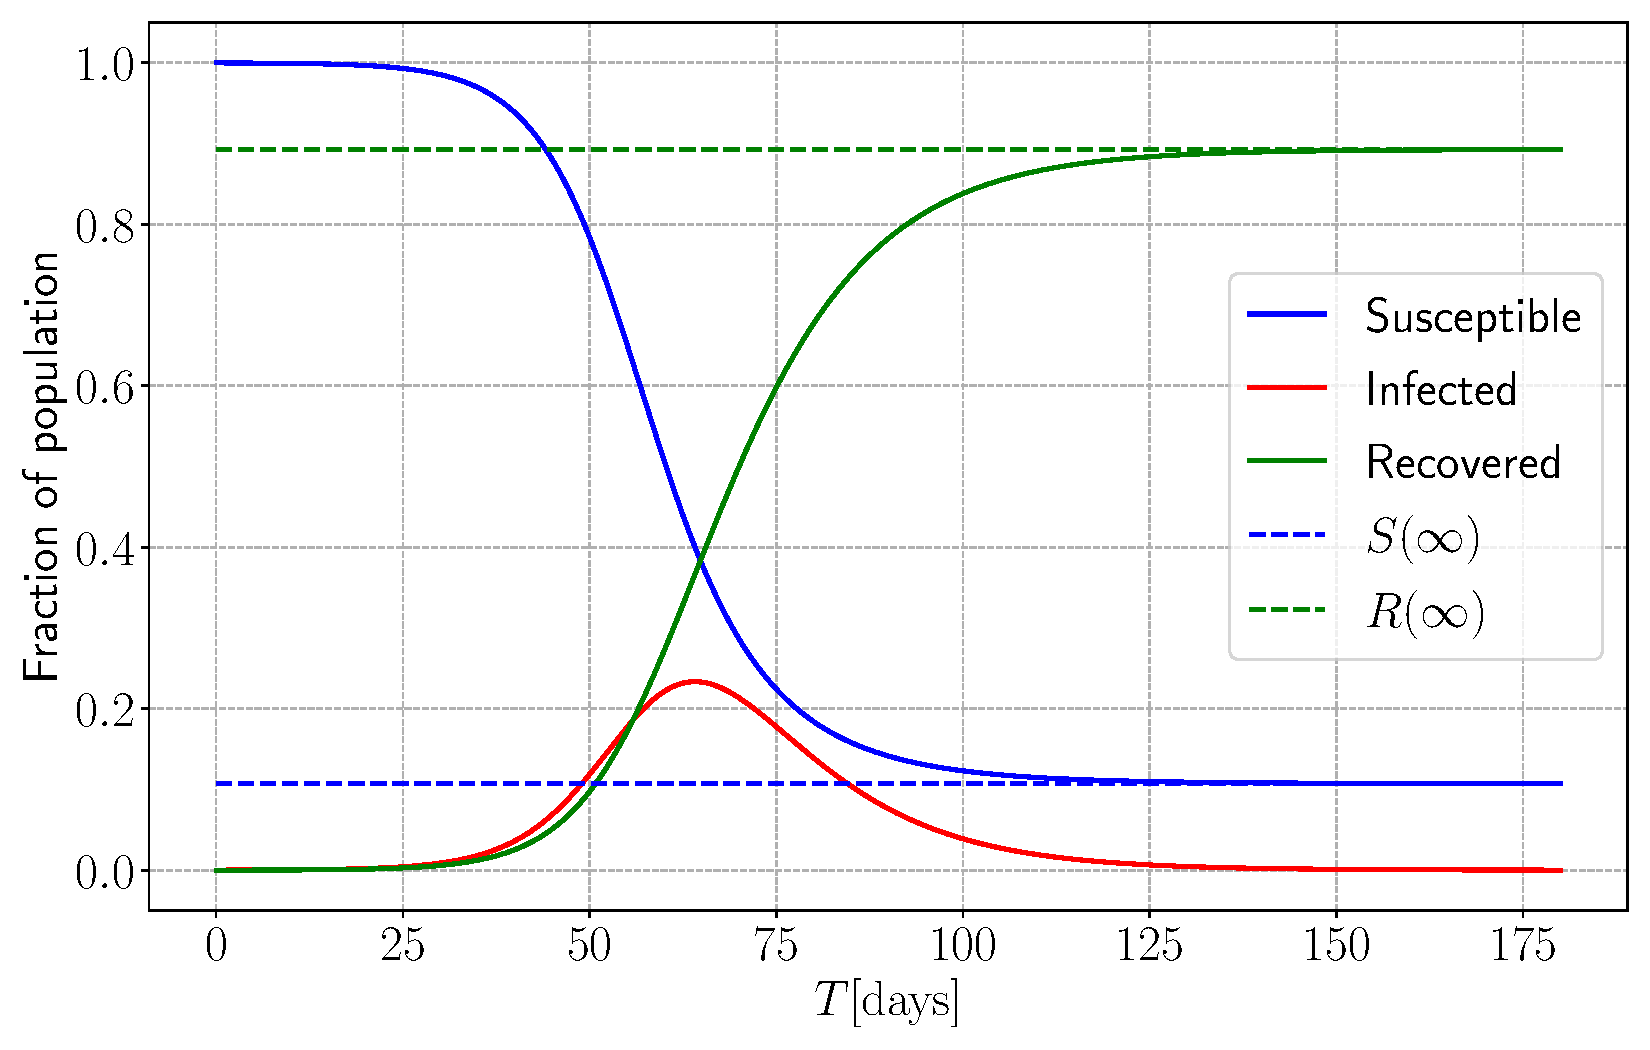
\includegraphics[width=0.8\columnwidth]{../fig/2Aa_SIR.pdf}
	\caption{SIR equations with $\beta = 0.25 \, \mathrm{day}^{-1}$, $\tau = 10 \, \mathrm{day}$.}
	\label{fig:SIR}
\end{figure}

\subsection{b)}

For the early developments of the epidemic, the expression for $I$ can be simplified to \cite{sheet}
\begin{equation}\label{eq:I_simp}
	\der{I}{t} = (\beta - 1/\tau) I.
\end{equation}
The solution of this equation is given by
$$
	I(t) = I(0) \exp{\left(\left[ \beta \tau - 1 \right] \frac{t}{\tau}\right)} = I(0) \exp{\left(\left[ \mathcal{R}_0 - 1 \right] \frac{t}{\tau} \right)},
$$
where we have introduced $\mathcal{R}_0 = \beta\tau$. As seen in figure \ref{fig:Infected}, the fraction of infected people matches this expression quite closely during the first $40$ days or so. This confirms the exponential growth in the beginning. 

\begin{figure}[htb]
	\centering
	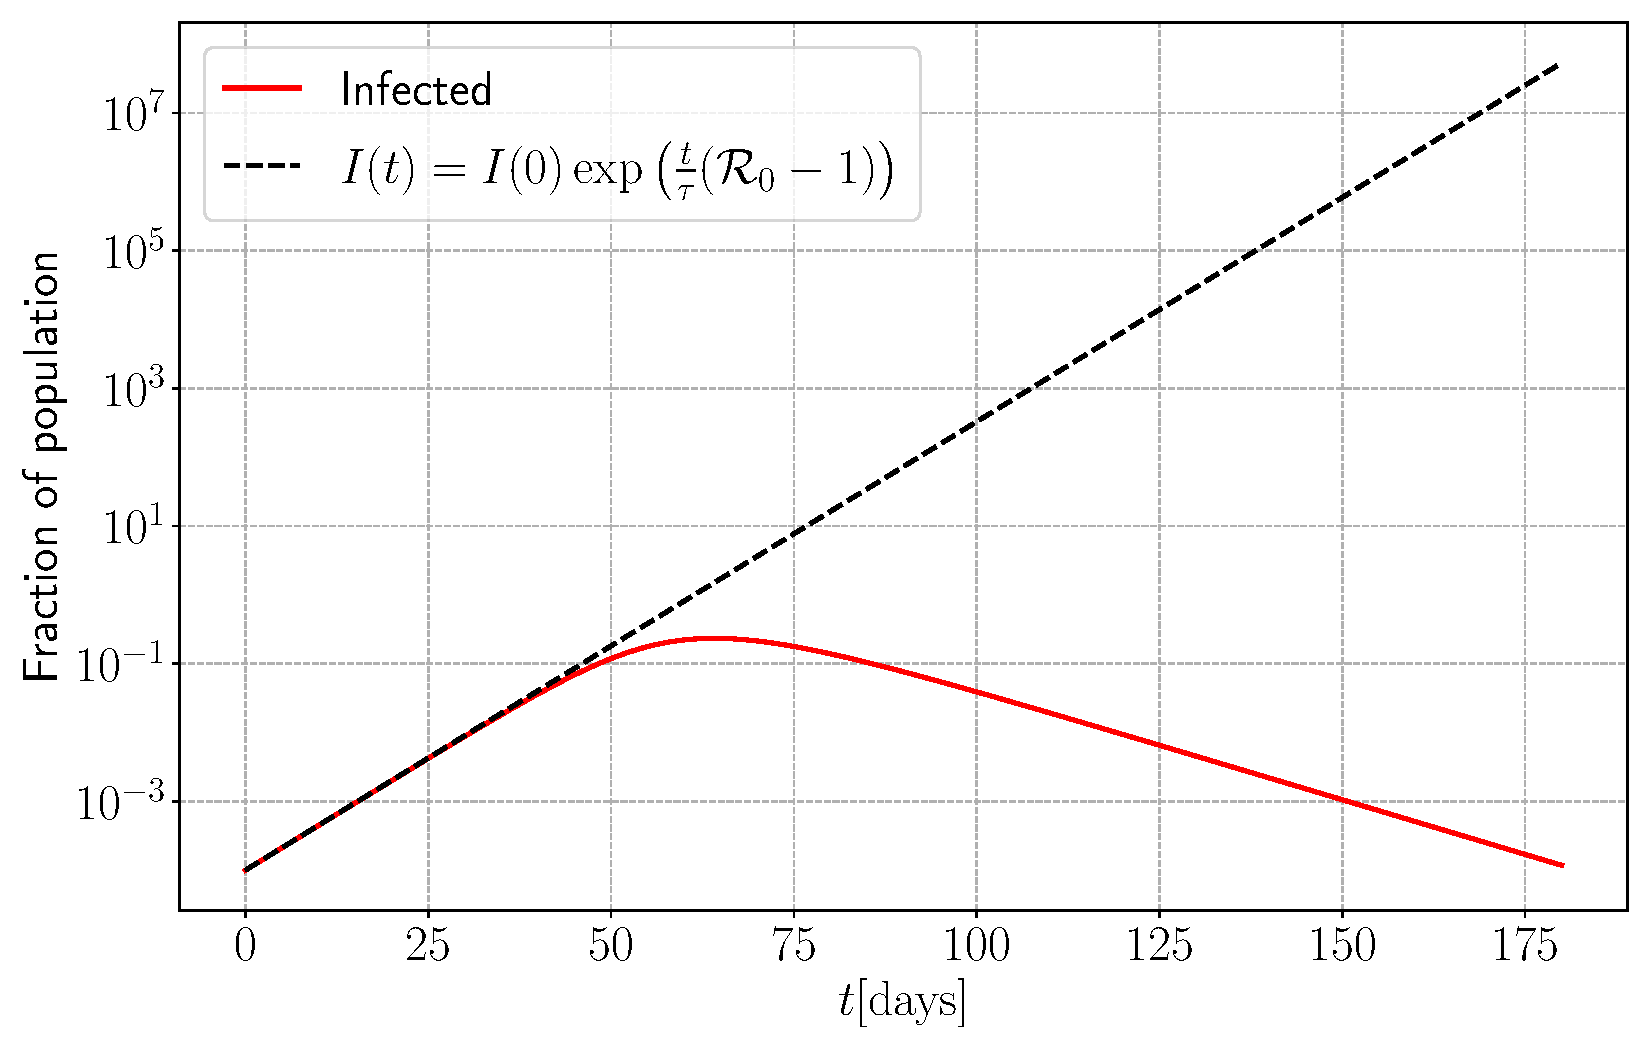
\includegraphics[width=0.8\columnwidth]{../fig/2Ab_I.pdf}
	\caption{Infected people compared with the analytical approximation at the early stages.}
	\label{fig:Infected}
\end{figure}

\subsection{c) Flattening the curve. }

As seen from figure \ref{fig:SIR}, the peak of the infected people is rather close to being at $0.2$ when $\beta = 0.25$. Remark also that the peak occurs in the early stage of the epidemic. We use these observations to our favour when finding the \textit{largest} $\beta$ that will keep $I/N$\footnote{Note that I use fractions of people instead of actual numbers of people in this section, so that is why I refer to $I$ as if it is $I/N$ in the procedure below.} smaller than $0.2$ during the pandemic. To do this, I choose the following procedure:

\begin{algorithm}[H]
	Choose a starting value for $\beta = \beta_0$\;
	Choose a tolerance $\texttt{tol}$\;
	Run the simulation of the SIR with the same parameters as in 2Aa, except with $\beta = \beta_0$.\;
	Calculate $\mathcal{I} \coloneqq \max_{t\in[0,180]} I(t)$.\;
	\While{\texttt{err }$\coloneqq | \mathcal{I} - 0.2 | > \texttt{tol}$}{
		\eIf{
			$\mathcal{I} > 0.2$
			}
			{$\beta\gets \beta \cdot 2^{\texttt{err}}$}
			{$\beta\gets \beta \cdot 2^{-\texttt{err}}$}	
		}
		Run the simulation of the SIR with the same parameters as in 2Aa, except with the new value for $\beta$.\;
		Recalculate $\mathcal{I} \coloneqq \max_{t\in[0,180]} I(t)$.\;
	\caption{Finding the largest beta keeping $\max I$ \textit{less} than 0.2.}
\end{algorithm} 

This procedure is by no means any advanced piece of algorithm, but it ensures that $\beta$ is increased when the maximum of $I$ is less than $0.2$, and decreased when it is larger than $0.2$. Further, it also ensures that the "nudging" of beta in each step is less when the error is less. To get an estimate for the \textit{largest} $\beta$ one can have to keep $I/N$ \textit{less} than $0.2$, one should start off with an initial value $\beta_0$ for which the peak is less than $0.2$, so that one reaches the limit from below. Using $\beta_0 = 0.2$, one finds with the maximum value of $\beta = 0.28020370$, as given in table \ref{tab:2Acd} together with the deviation $0.2 - \max_{t\in[0,180]} I(t)$ this value gives rise to.  


%\begin{figure}[htb]
%	\centering
%	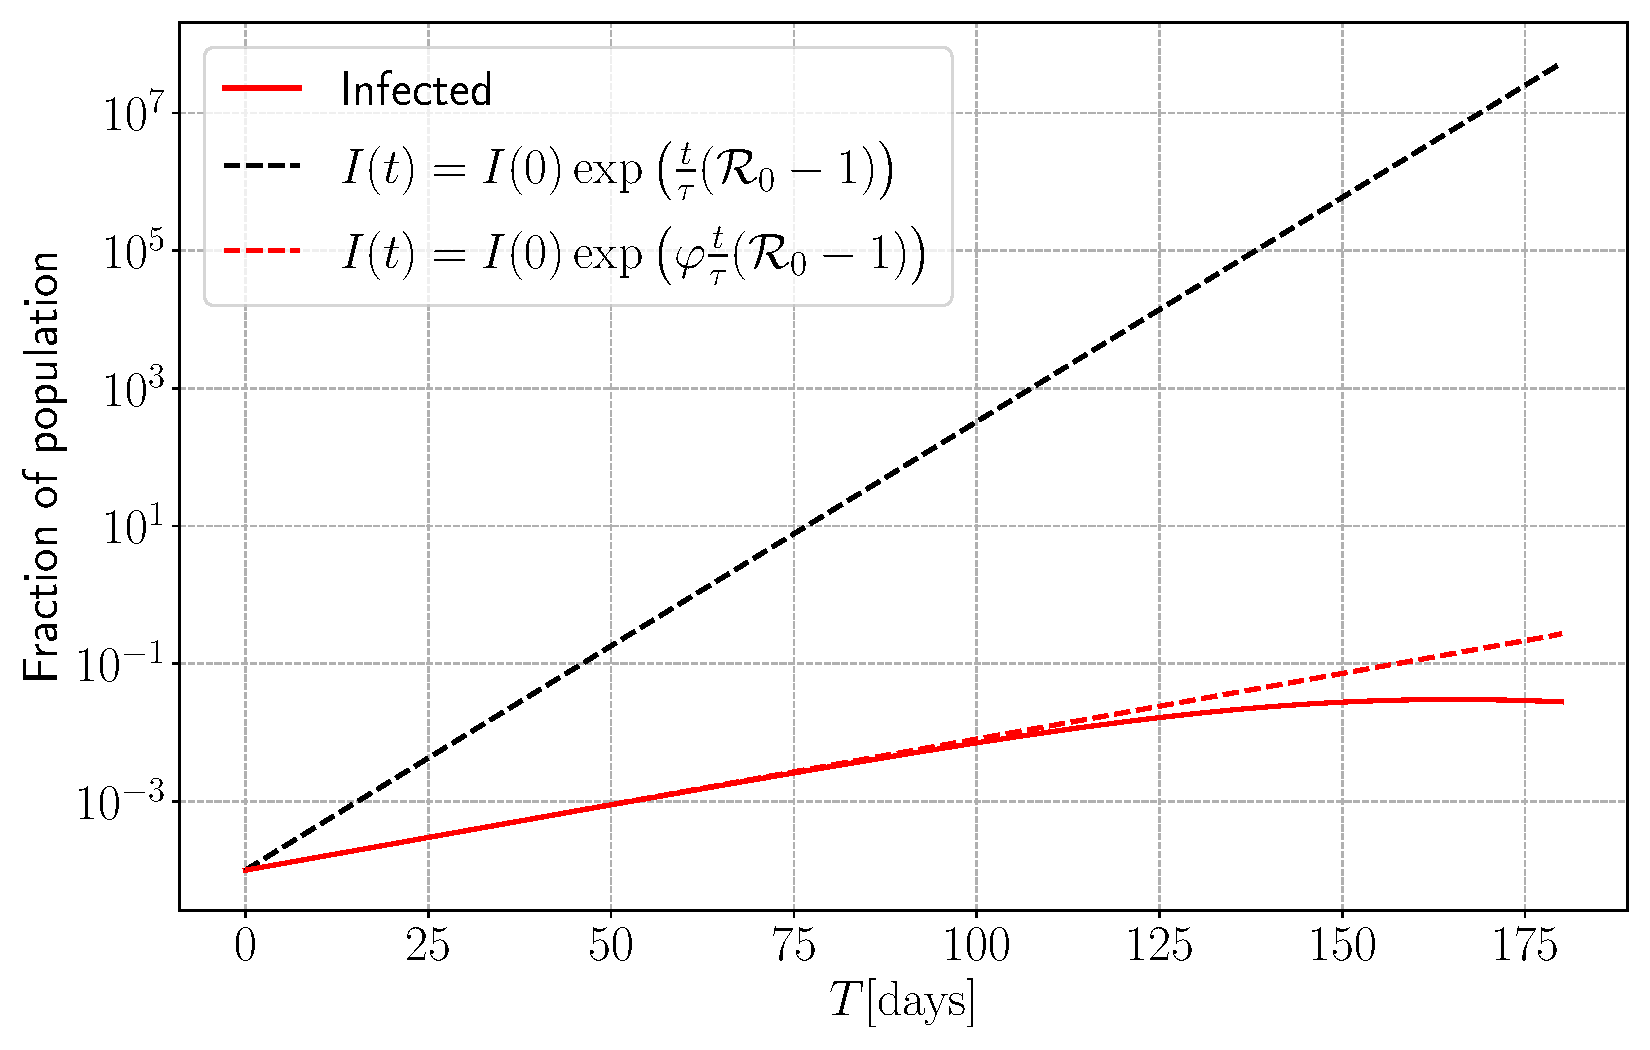
\includegraphics[width=0.8\columnwidth]{../fig/vac.pdf}
%	\caption{The effect of vaccination, with $\varphi = 0.3$.}
%	\label{fig:vaccination}
%\end{figure}

\subsection{d) Vaccinations}

To find the minimum fraction of vaccinated people preventing an outbreak, $R(0)/N$, I use the following procedure:

\begin{algorithm}[H]
	Choose a starting value for $R(0) = R_0$\;
	Run the simulation of the SIR with the same parameters as in 2Aa, except with $R(0) = R_0$ \;
	Calculate the \texttt{slope} of the fraction of infected people in a semi-log plot for the first $15$\footnote{As people are typically sick for $10$ days ($\tau = 10$) I regard this time scale as long enough to detect whether the outbreak grows exponentially or decays.} days of the simulation\;
	If the initial slope is negative it indicates that the outbreak dies out by itself\;
	\While{\texttt{slope}$ > 0$}{
		$R(0) \gets R \cdot 2 ^{\texttt{slope}}$ \;
	Run the simulation of the SIR with the same parameters as in 2Aa, except with the new value for $R(0)$.\;
	Recalculate the \texttt{slope} in the semi-log axes.\;}
	\caption{Finding the minimum fraction of initially vaccinated people for outbreaks to be impossible.}
\end{algorithm} 

The value of $R(0)/N$ preventing an outbreak found from this procedure is $0.59987499$, as shown in table \ref{tab:2Acd} together with the slope in the semi-log plot which this fraction yields for $I(t)$. This is obtained from running the procedure with $R_0 = 0.1$.

\begin{table}[htb]
	\centering
	\caption{The maximum value of $\beta$ giving a peak less than $0.2$ of the infected fraction, and the minimum value of $R(0)$ (vaccinated) avoiding exponential growth.}
	\begin{tabular}{cccc}
		\toprule
		Parameter & value & $0.2 - \max_{t\in[0,180]} I(t)$ & Initial $\log$-slope \\
		\midrule
		$\beta$ & $0.28020370$ & $8.319\cdot 10^{-7}$ & --- \\
		$R(0)$  & $0.59987499$ & --- & $-1.74\cdot 10^{-15}$ \\
		\bottomrule
	\end{tabular}
	\label{tab:2Acd}
\end{table}


\clearpage

\section{Problem 2B: Stochastic SIR model}


\begin{figure}[htb]
	\centering
	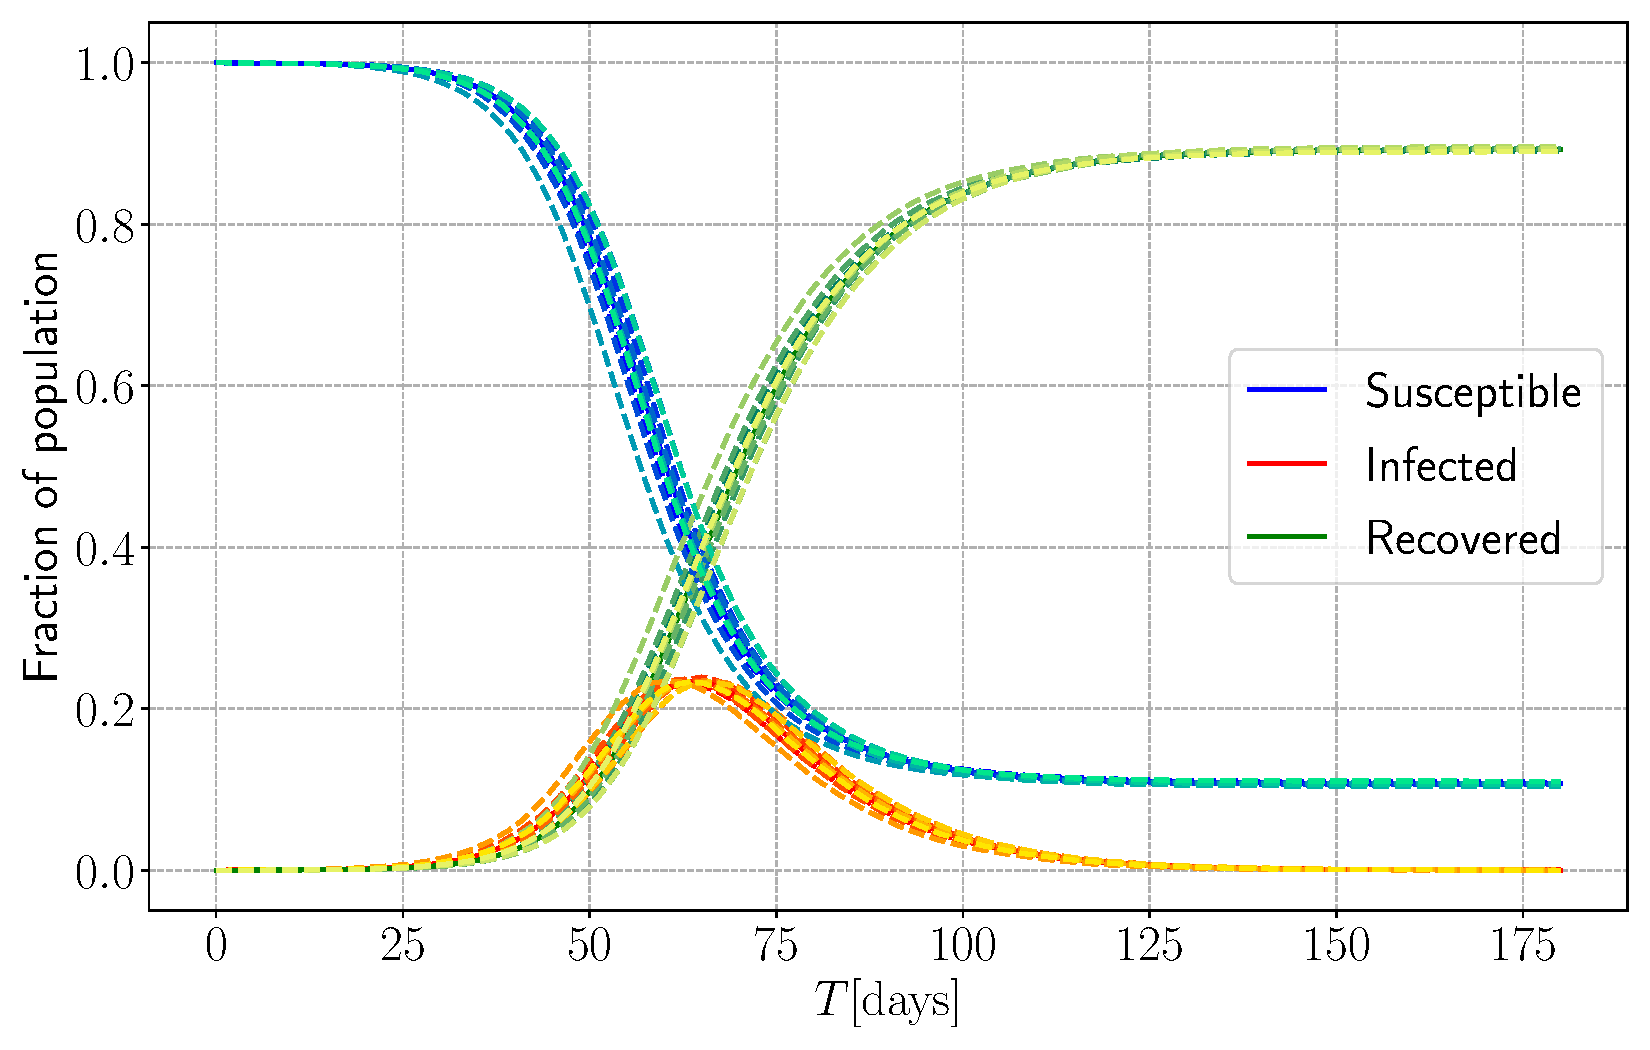
\includegraphics[width=0.8\columnwidth]{../fig/2Ba_SIR.pdf}
	\caption{Solution of stochastic SIR equations with $\beta = 0.25\, \mathrm{day}^{-1}$, $\tau = 10\, \mathrm{day}$.}
	\label{fig:SIR_stoch}
\end{figure}

\begin{figure}[htb]
	\centering
	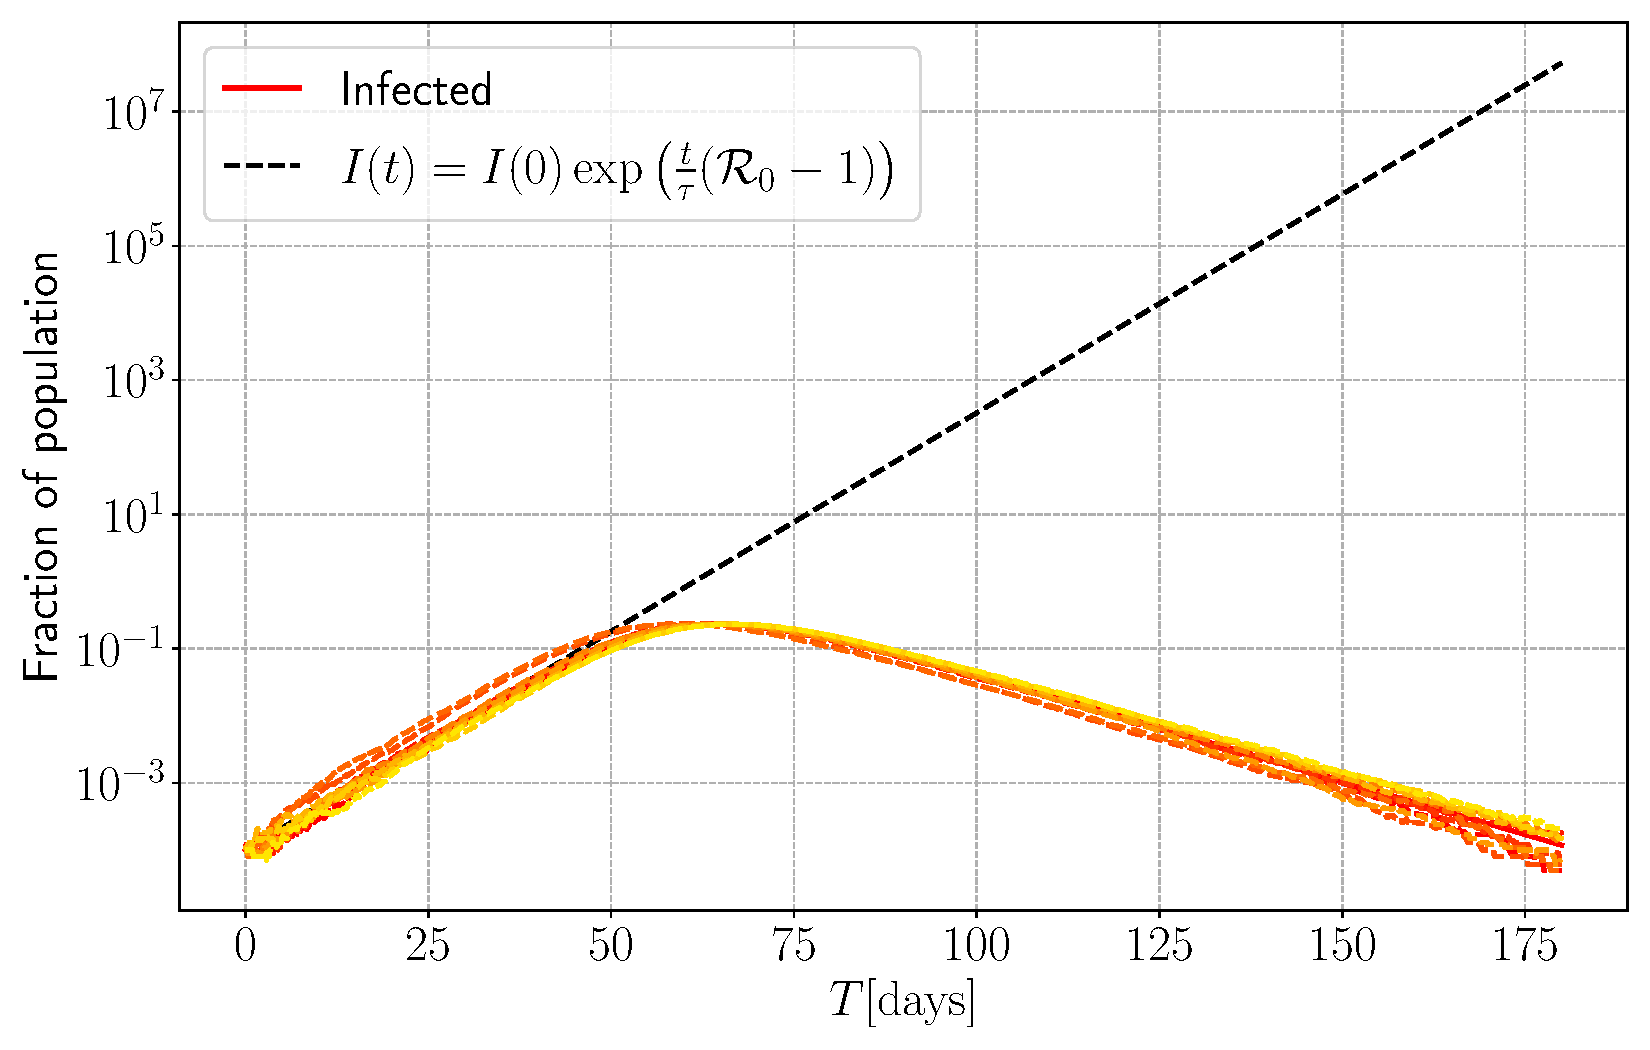
\includegraphics[width=0.8\columnwidth]{../fig/2Bb_I.pdf}
	\caption{Infected people compared with the analytical approximation at the early stages. Stochastic and continuous model.}
	\label{fig:Infected_stoch}
\end{figure}


\begin{figure}[htb]
	\centering
	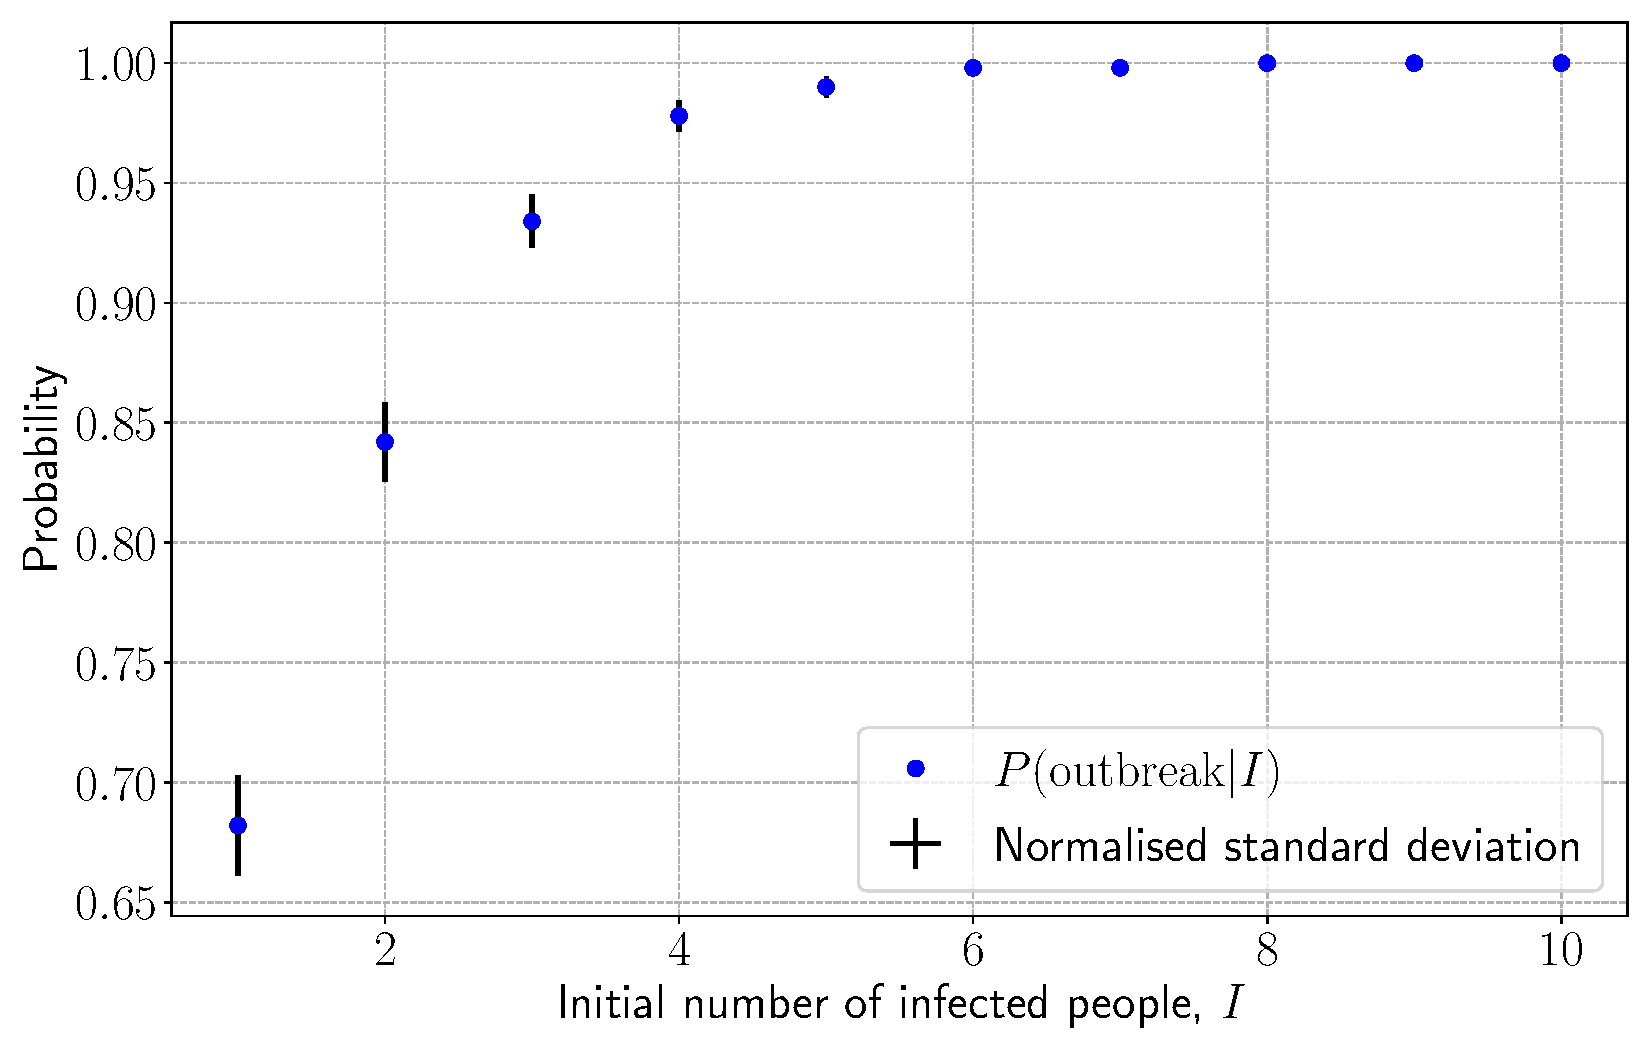
\includegraphics[width=0.8\columnwidth]{../fig/2Bc_prob.pdf}
	\caption{Probability of an outbreak as a function of initial number of infected people.}
	\label{fig:prob_outbreak}
\end{figure}
\section{Problem 2C: Stochastic SEIIaR model}

\subsection{a)}

The time-development of all the variables in the SEIIaR model is shown in figure \ref{fig:SEIIaR}, showing $10$ realisations of the simulation. To compare it easily with the deterministic model, we contract $E,I,I_a$ into one variable, so that they together represent all the infected people. The solutions of the deterministic model are shown together with the contracted versions of these simulations in figure \ref{fig:SEIIaR_compare}. 

\begin{figure}[htb]
	\centering
	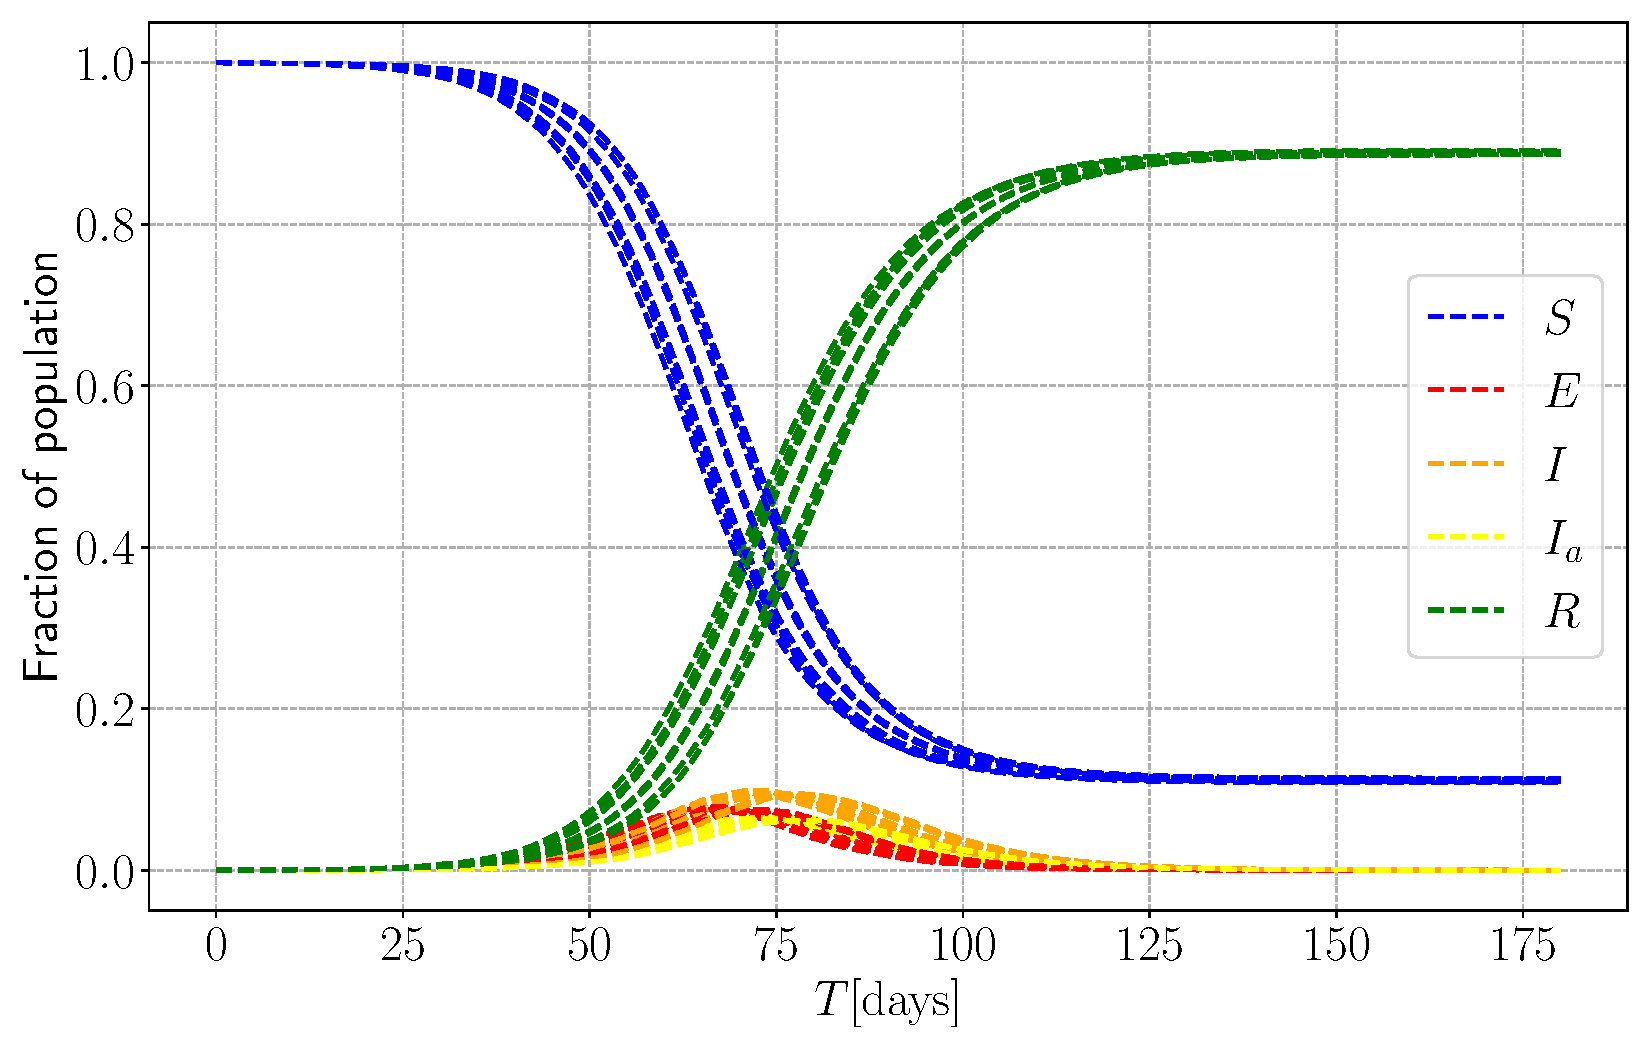
\includegraphics[width=0.8\columnwidth]{../fig/2Ca_SEIIaR.pdf}
	\caption{Solution of the stochastic SEIIaR-equations.}
	\label{fig:SEIIaR}
\end{figure}

\begin{figure}[htb]
	\centering
	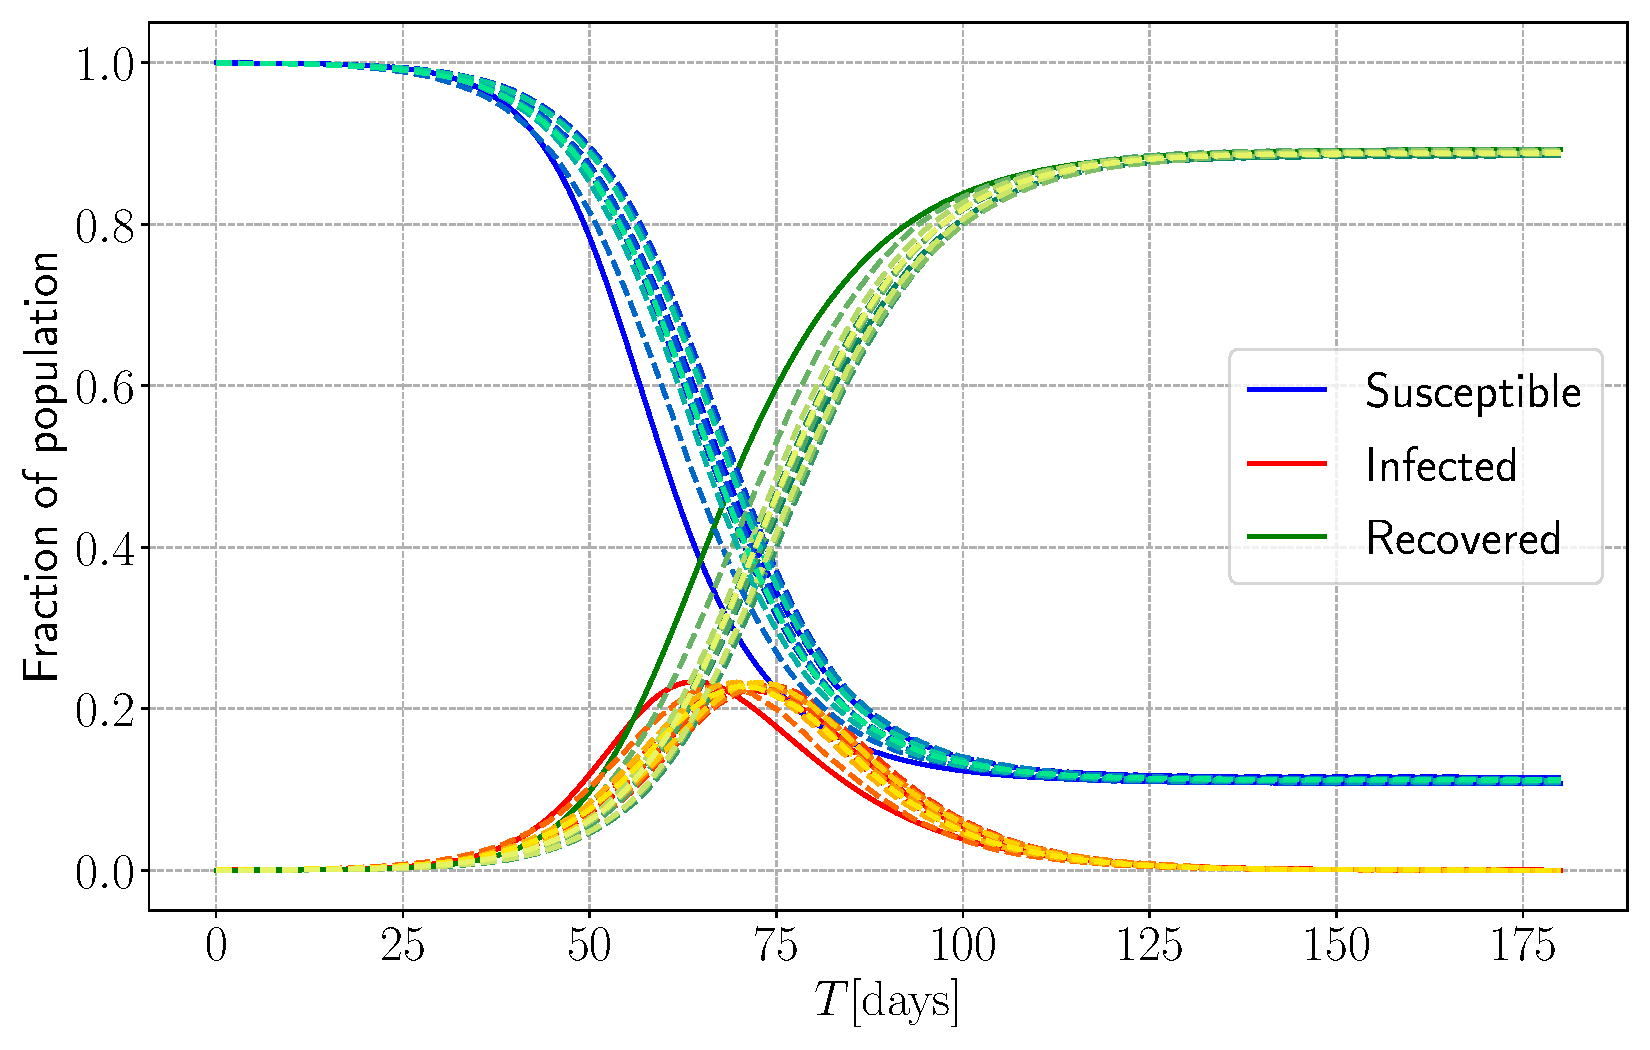
\includegraphics[width=0.8\columnwidth]{../fig/2Ca_comp.pdf}
	\caption{Comparison of the solution of the Stochastic SEIIaR-equations with the deterministic SIR-model. The number of infected people $I$ in the stochastic model is $E + I + I_a$.}
	\label{fig:SEIIaR_compare}
\end{figure}

One prominent feature to notice here, is that the process overall seems to be \textit{slower}, in the sense that it takes longer for people to get infected and eventually recover, but the peaks and asymptotic behaviours seem to align quite closely. This is probably due to the fact that this model includes a period in which people are infected but not yet able to infect anybody else, an incubation period of typical length $\tau_E = 3 \, \mathrm{days}$. This will naturally delay the process, but it should not affect the peak nor the asymptotic behaviour. Ultimately, this shows that the SEIIaR model adds another layer of realism to our model in the sense that people do not get sick right away. Another thing to mention is that the fraction of infected asymptomatic people $I_a$ are always less than the fraction of infected symptomatic people $I$. This is as expected since $f_a < f_s$, and the probabilities of transitioning to either of these states are the same.

To test that the implementation is correct --- by comparing with the deterministic and stochastic SIR model --- we adjust the parameters of the SEIIaR to $\beta = 0.25$, $r_s = 1$, $r_a = 1$, $\tau_E = 0$, $\tau_I= 10$ and start with $10$ out of $100 \, 000$ people initially infected. The results of doing $1000$ such simulations and performing the average of the stochastic models is shown in figure \ref{fig:comparison_SIR}. This shows that the two stochastic models are more or less identical, as expected.

\begin{figure}[htb]
	\centering
	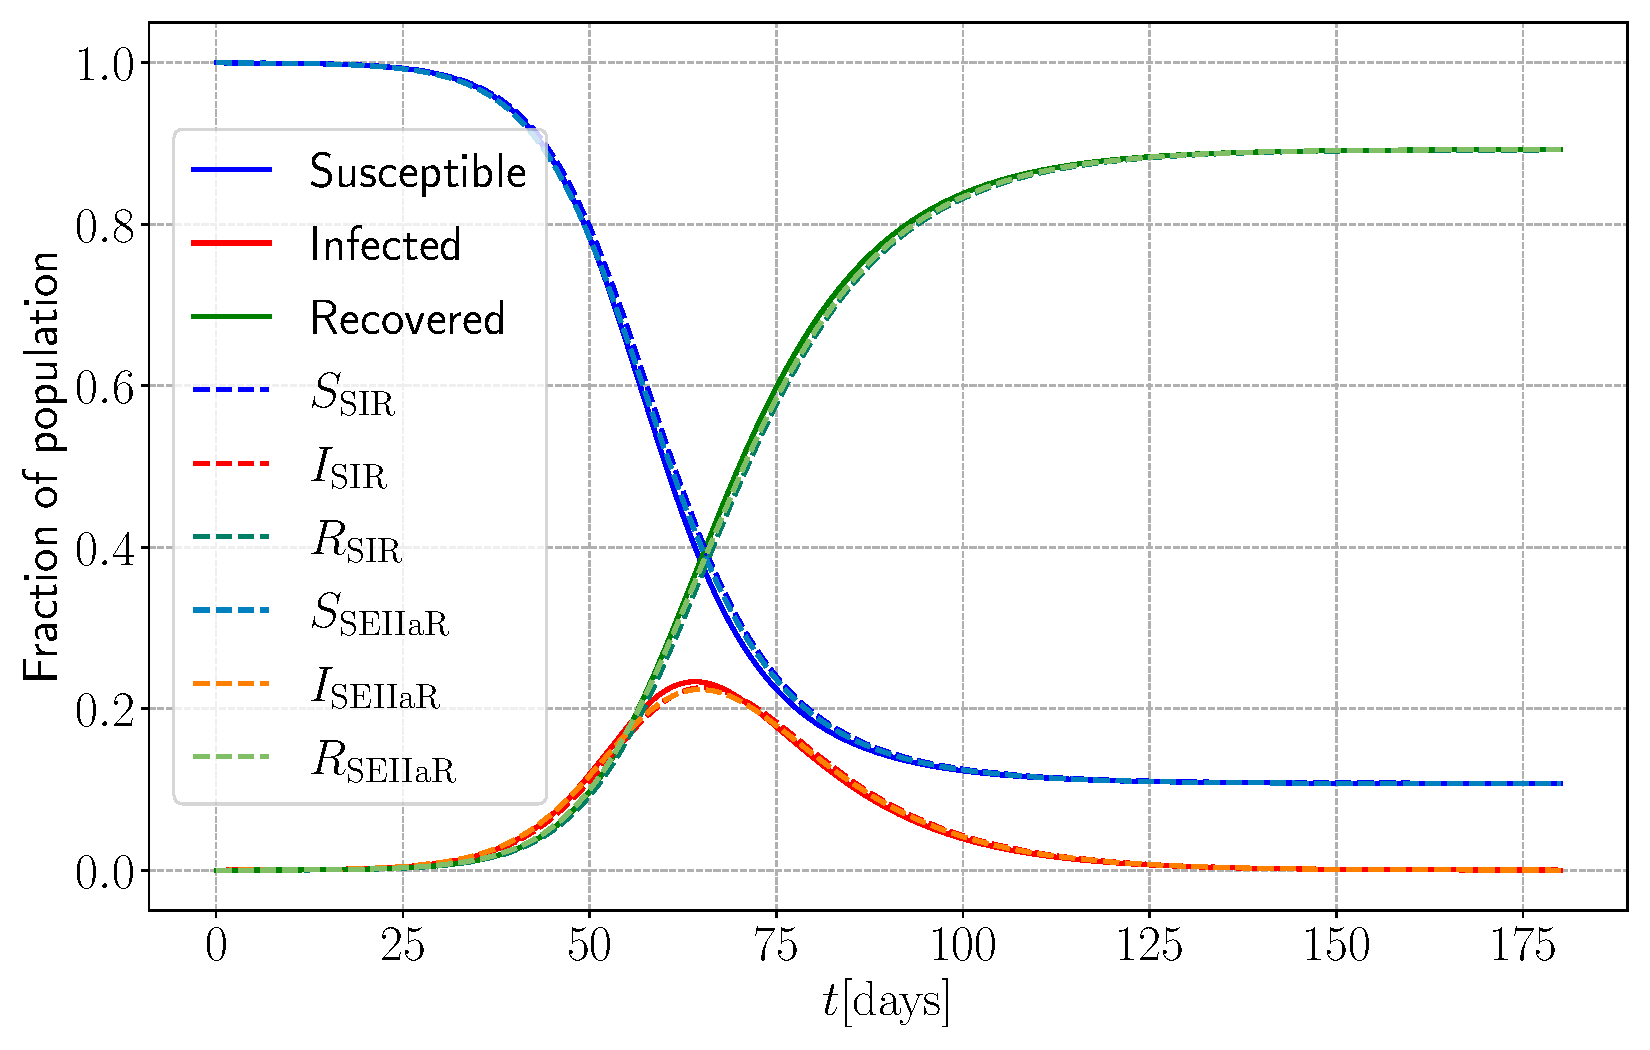
\includegraphics[width=0.8\columnwidth]{../fig/test_comparison.pdf}
	\caption{Solution of the stochastic SEIIaR-equations compared with the stochastic and deterministic SIR-equations for the case of identical parameters.}
	\label{fig:comparison_SIR}
\end{figure}

\subsection{b) Probability of outbreak dependence on $r_s$}

The variable $r_s$ describes how infectious a person is when he is in the infection state. Reducing this constant below $1$ can therefore correspond to emulating the degree of self-isolation when people are symptomatic. We investigate the probability of an outbreak as a function of this self-isolation-rate $r_s$ by the following procedure (which is essentially the same as that shown in $2Bb$ expect we are now finding the probability as a function of $r_s$): 

\begin{algorithm}[H]
	Choose the parameters of the model as those given in the exam sheet \cite{sheet}, but with $T = 30 \, \mathrm{days}$\footnote{As the typical infection time is still $10$ days, I assume 50 days to be more than sufficient for detecting an outbreak in the stochastic model.}. \;
	Choose a batch-size $B$.\;
	Choose a number of values $n$ of $r_s$ to try\;
	Select $n$ values of $r_s$, equally spaced between $0.001$ and $1$ :
		$$
			\mathbf{R} = [R_1, \dots R_n]
		$$
	\For{$i = 1,2,\dots, n$}{
		Initialise an empty vector of length $B$: $\mathbf{X} = [0,\dots,0]$.\;
		\For{$n = 1,\dots, B$}
		{
			Run the simulation with $r_s = R_i$.\;
			Calculate the \texttt{slope} in the semi-log axes for $I(t)$.\;
			\eIf{$\texttt{slope} <= 0$}
			{$X_n = 0$}
			{$X_n = 1$}
		}
		Estimate the probability of an outbreak for $I$ initially infected by 
		$$
		p \coloneqq P(\mathrm{outbreak}|r_s) = \frac{1}{B} \sum_{n= 1}^{B} X_n. \;
		$$	
		Calculate the standard deviation of the estimate by 
		$$
		\sqrt{\mathrm{Var}(\hat{p})} = \sqrt{\frac{p(1-p)}{B}}.
		$$
	}
	\caption{Calculating the probability of an outbreak as a function of $r_s$.}
\end{algorithm} 

The results of this calculation using a batch size of $B = 500$ and $100$ values of $r_s$ are shown in figure \ref{fig:rs_prob}. The behaviour is as expected: when people are hardly infectious when symptomatic the probability of an outbreak is close to $0$. This is also probably also a result of the fact that $r_a = 0.1$, i.e. it is not particularly likely to infect anyone when you are asymptomatic. If $r_a$ and $f_a$ was higher, one would expect the probability distribution to stagnate at some finite value when $r_s \to 0$, or at least go to $0$ slower. This is demonstrated in the same figure, where we set $r_a = 1$ and perform the same test as above. This again is an intuitive confirmation that the model behaves as expected, and therefore is correctly implemented.

\begin{figure}[htb]
	\centering
	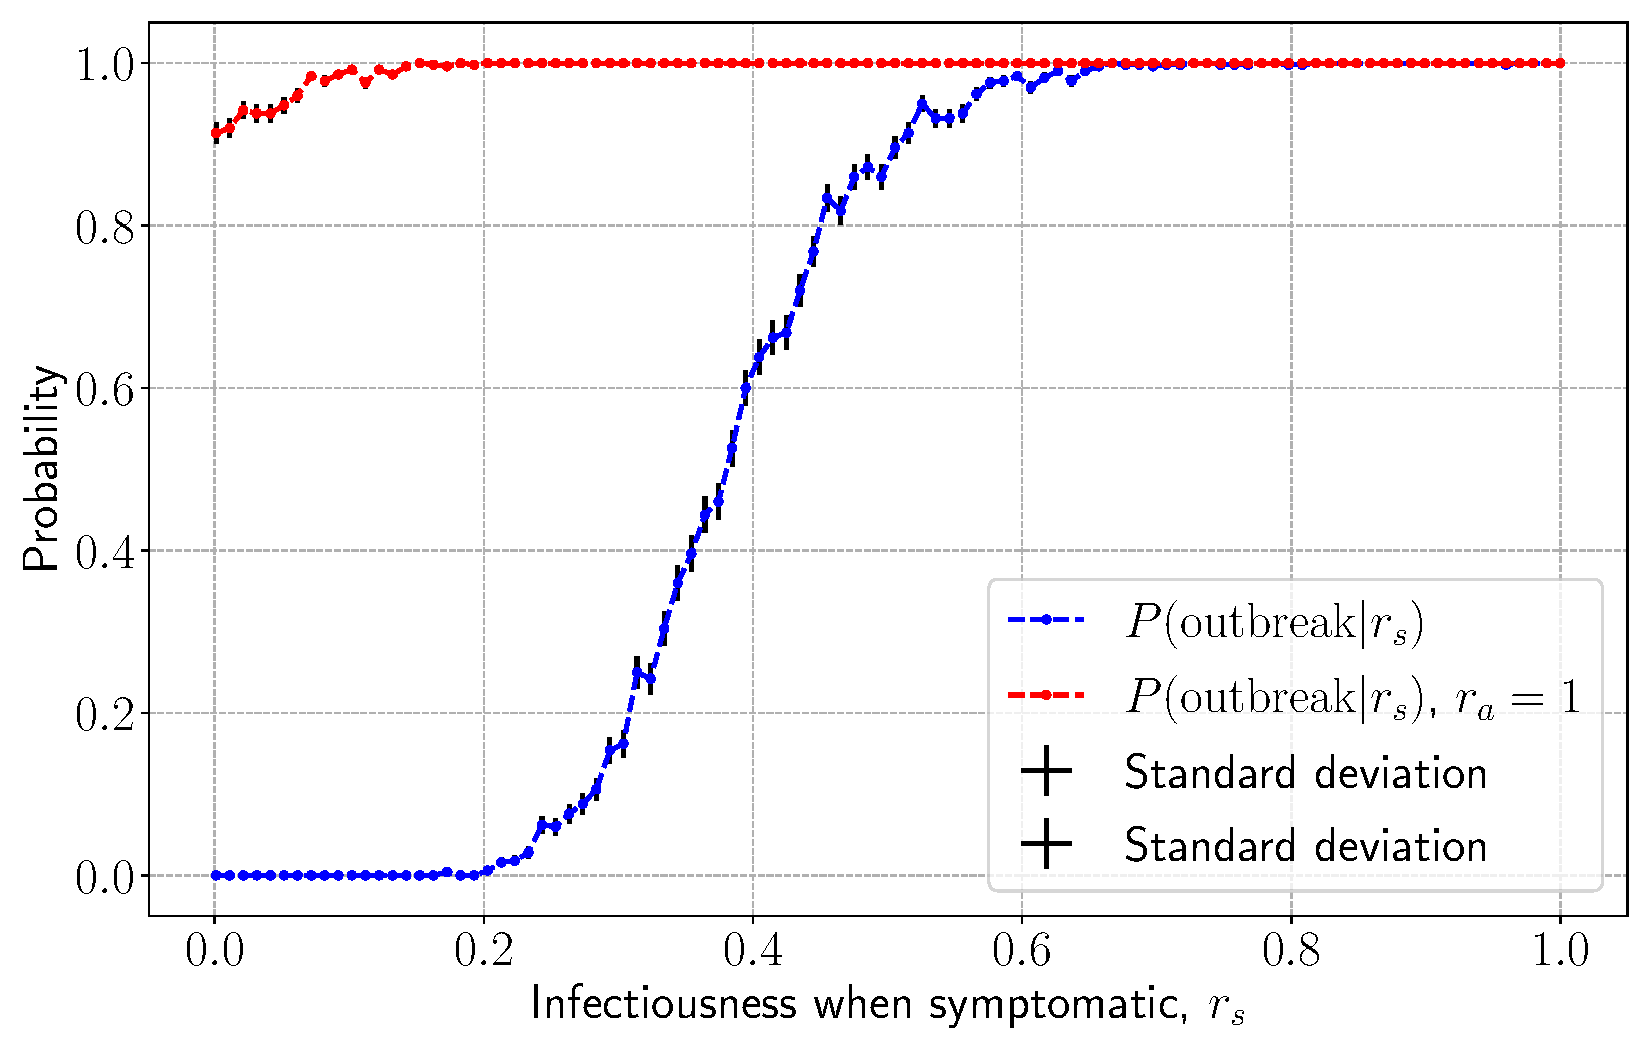
\includegraphics[width=0.8\columnwidth]{../fig/2Cb_probs.pdf}
	\caption{Probability of an outbreak as a function of $r_s$.}
	\label{fig:rs_prob}
\end{figure}


\clearpage
\section{Problem 2D: Stochastic SEIIaR Commuter model}

\subsection{a) Commuter model for a two-town system}

I set up a population structure as described by the matrix 
$$
	\mathbf{M} = \begin{bmatrix}
	9000 & 1000 \\
	200 & 99800
	\end{bmatrix},
$$
and simulate the time evolution of each of the five states for $180$ days, as described in \cite{sheet}, with $25$ initially exposed people working and living in town $1$. The results of this simulation is shown in figure \ref{fig:commuter_2city}. Notice that we here use the number of people as scale on the vertical axis, so that we easier can distinguish the two towns from each other. We observe that the evolution of the epidemic in town $2$ is delayed compared to that of town $1$. This is as expected, as only $25$ people in town $1$ are exposed, and they can only infect people in town $2$ \textit{via } someone that works in town $2$. 

Also here, note that at each time there are fewer asymptomatic infected than symptomatic infected. This is as expected since $f_a < f_s$, and the probability of transitioning to either of these states are equal.  

\begin{figure}[htb]
	\centering
	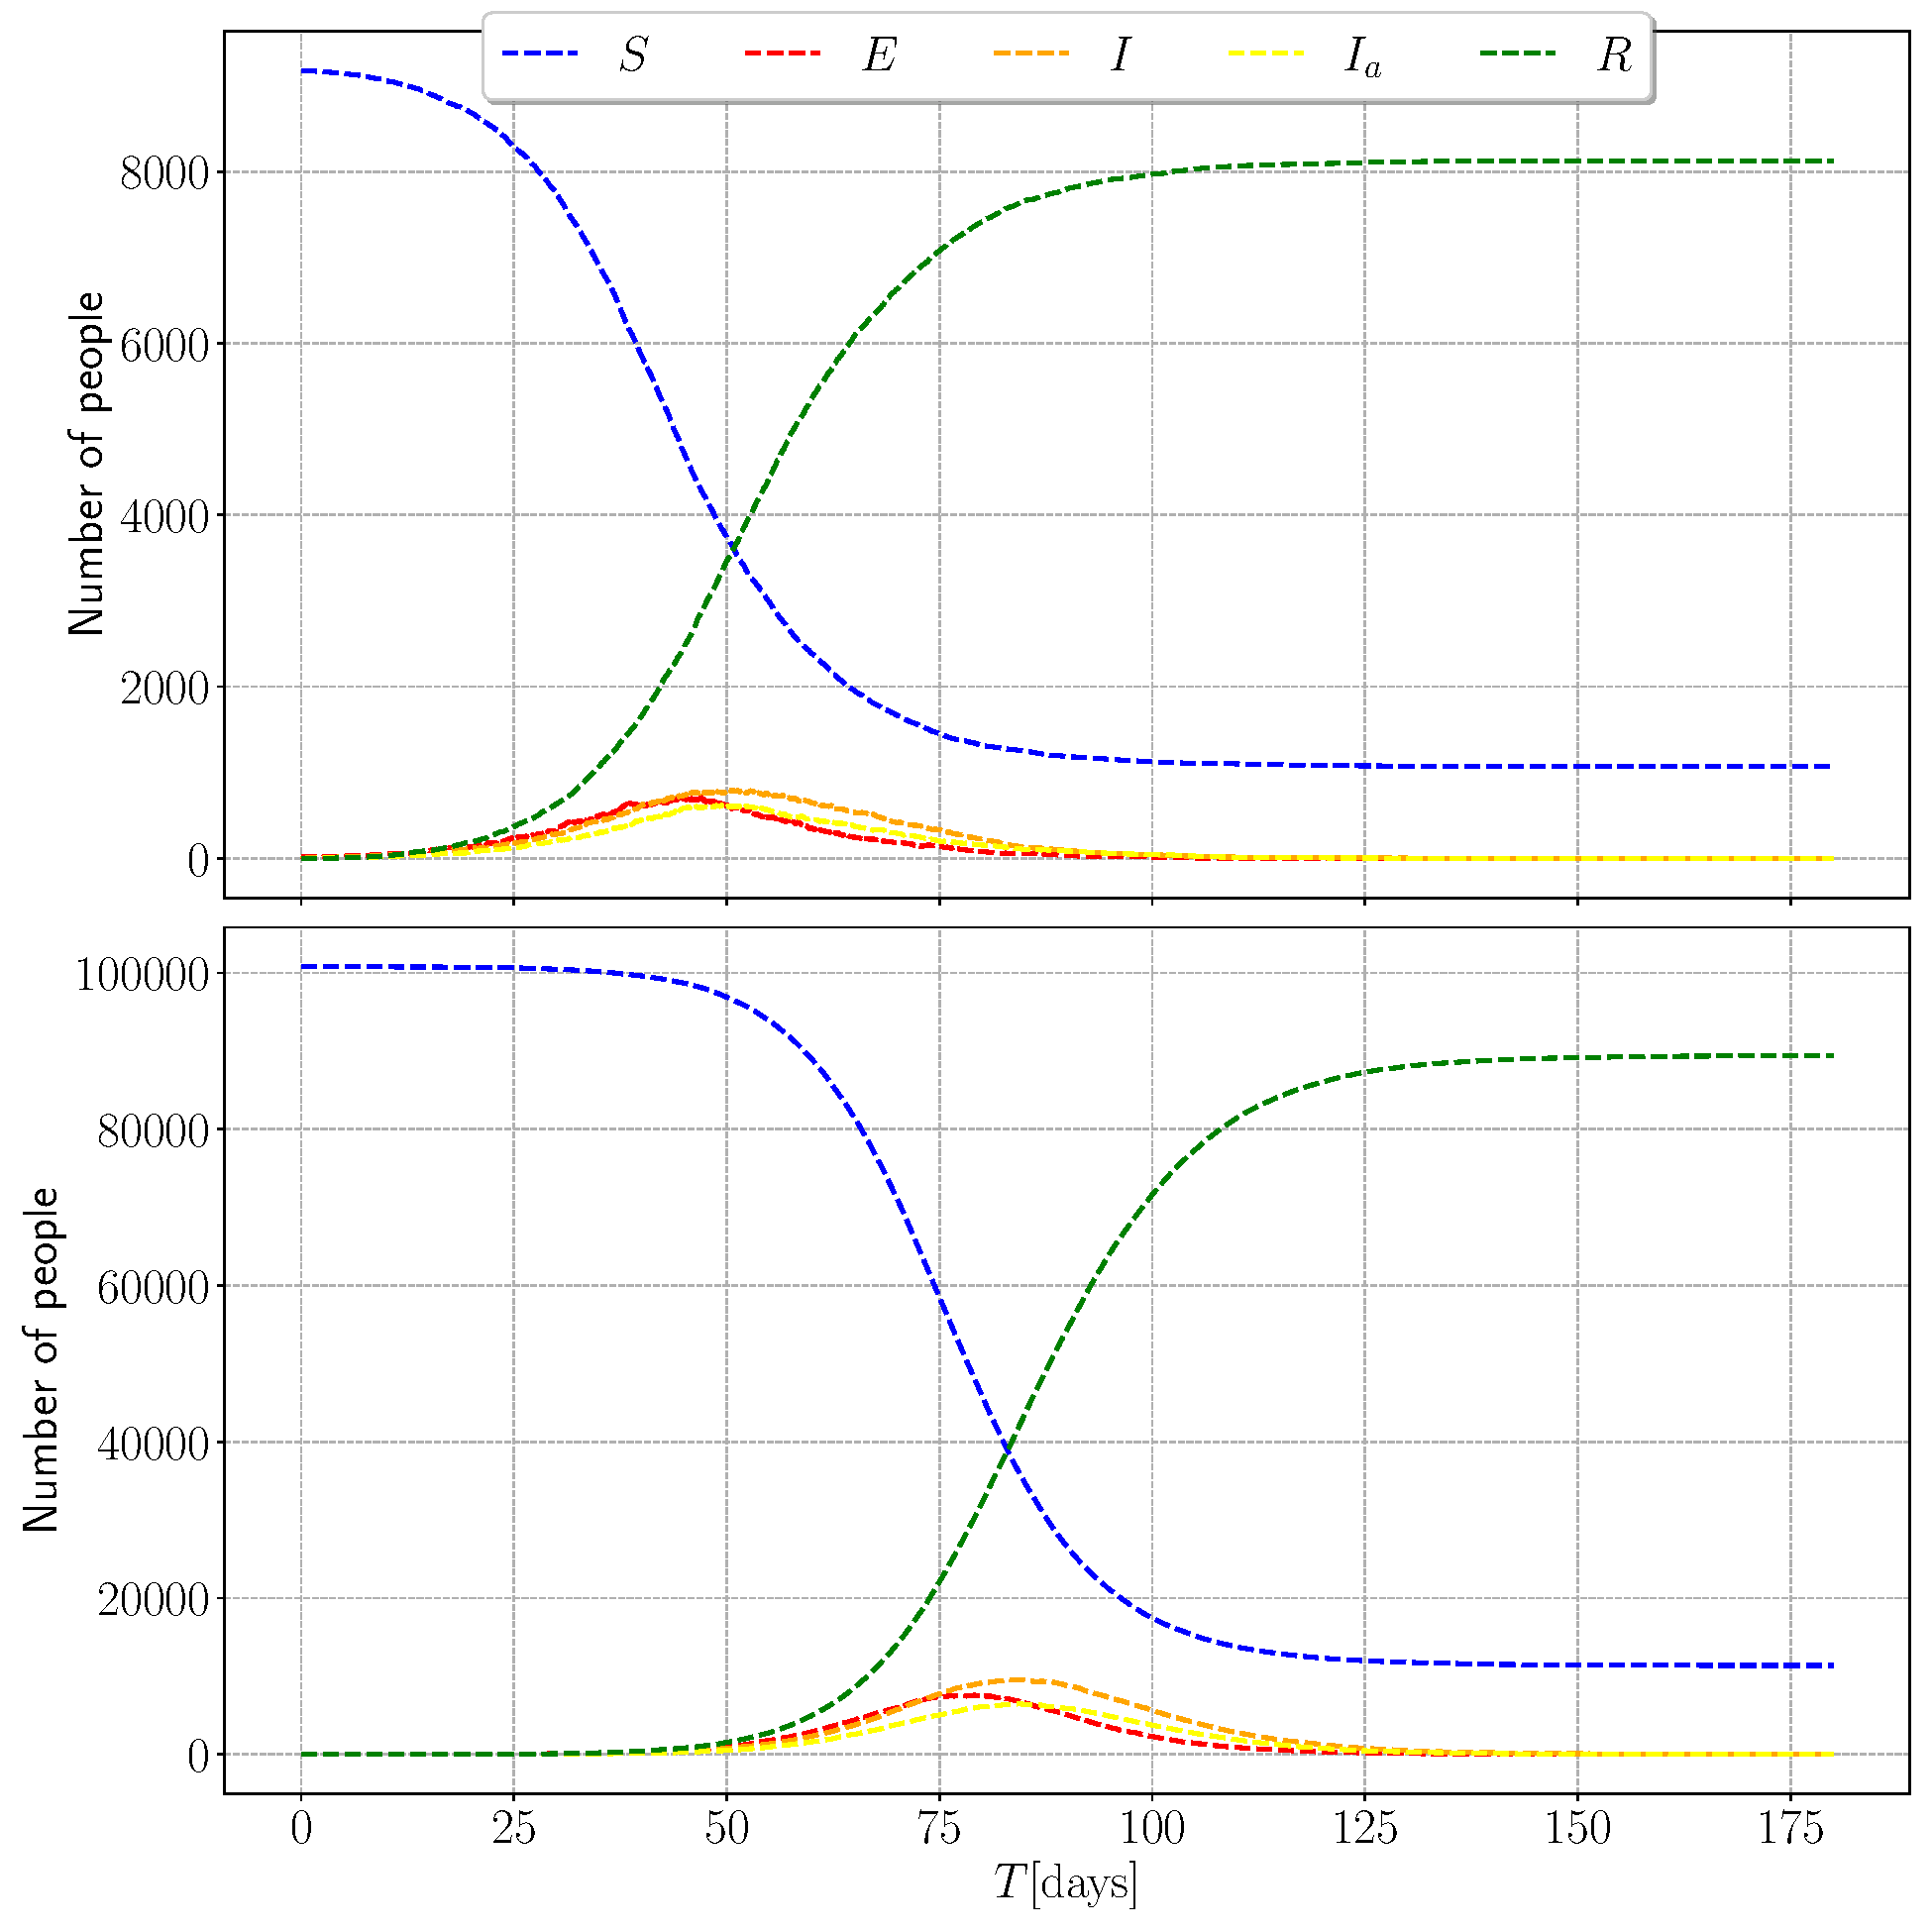
\includegraphics[width=0.8\columnwidth]{../fig/2Da_commuter.pdf}
	\caption{Solutions of Stochastic SEIIaR commuter model for the $2$-city case.}
	\label{fig:commuter_2city}
\end{figure}

\subsection{b) Description of implementation \& tests} 

To implement the Stochastic SEIIaR Commuter model, I choose the following procedure: 

\begin{algorithm}[H]
	Choose a population structure $\mathbf{M} \in \mathbb{N}^m \times \mathbb{N}^m$, i.e. an $m\times m$ matrix\;  
	Set an end time $t_N$ and a time-step $\Delta t$\;
	Set an initial state $\mathbf{X}_0 \in \mathbb{N}^m \times \mathbb{N}^m \times \mathbb{N}^5$, where entry $X_{0,ij}$ is the vector $\mathbf{v}$ of the variables $S,E,I,I_a,R$ for group $(i,j)$ in the matrix $\mathbf{M}$.\;
	Create an empty array for holding the state at each point in time, $\mathbf{X}$, and set its first element to $\mathbf{X}_0$.\;
	Calculate the probabilities:
	\begin{align*}
		P_{E\to I} &= f_s \times (1 - \exp{(-\Delta t/\tau_E)}) \\
		P_{E\to I_a} &= f_a \times (1 - \exp{(-\Delta t/\tau_E)}) \\
		P_{I\to R} = P_{I_a\to R} &= 1 - \exp{(-\Delta t/\tau_I)} 
	\end{align*}
	Calculate the number of days $D = \texttt{int}(t_N)$, and the number of steps per half day $S = \texttt{int}(1/(2\Delta t))$.\; 
	\For{$d = 0,\dots, D - 1$}
		{
		$i \gets 2 \times d \times S$\;
		\For{$j = 0,\dots, S - 1$}
			{
			Calculate the number of people in each town, $\beta$,
				$$
				N_\beta = \sum_{\alpha = 1}^{m} M_{\alpha \beta} 
				$$ 
			Find the number of infected people of each kind at the previous time step for each town $\beta$,
				$$
				I_{\beta}, I_{a,\beta} = \sum_{\alpha = 1}^{m} X_{(i+j)\alpha\beta3},  \sum_{\alpha = 1}^{m} X_{(i+j)\alpha\beta4} 
				$$
			Calculate the probability for transitioning between $S$ and $E$ for each town, $\beta$, \footnote{Note that here I have used $\beta_0$ to denote the beta value describing the value of the model, to not confuse it with the summation variables.}
				$$
				P_{S\to E,\beta} = 1 - \exp{\left( - \Delta t \beta_0 \frac{r_s I_{\beta} + r_a I_{a,\beta}}{N}\right)} 
				$$
			}
			Do a normal SEIIaR step for each group of people $\alpha,\beta = 1,\dots,m$, exactly as described in the previous section.\;   
		$i \gets i + S$\;
		\For{$j = 0,\dots, S - 1$}
			{
			Repeat the procedure in the loop above, but with $\alpha \leftrightarrow \beta$, i.e. perform the sums over the \textit{third} not \textit{second} axis of $\mathbf{X}$, and the \textit{second} of $\mathbf{M}$. \;
			}
		}
		\caption{Description of implementation of the SEIIaR commuter model.}
\end{algorithm} 

Listing \ref{lst:commuter} shows the same algorithm as described above implemented in python.

\begin{lstlisting}[language=Python,label={lst:commuter},caption={SEIIaR commuter algorithm implemented in python}]
@nb.njit()
def SEIIaR_commuter_step(X,Pse,Pei,Peia,Pir,Piar):

    Dse          = np.random.binomial(X[0],Pse)
    Dei,Deia,Dee = np.random.multinomial(X[1], (Pei,Peia,1-Pei-Peia) )
    Dir          = np.random.binomial(X[2], Pir)
    Diar         = np.random.binomial(X[3], Piar)

    return np.array([X[0] - Dse,
                     X[1] - Dei - Deia + Dse,
                     X[2] - Dir + Dei,
                     X[3] - Diar + Deia,
                     X[4] + Dir + Diar])

@nb.njit()
def SEIIaR_commuter(M,X_0,tN,dt):
    
    # set this to ones initially, but change it 
    # for each step, as it depends on the number of infected.

    m    = np.shape(M)[0] 
    Pse  = np.ones(m)

    Pei  = fs * (1 - np.exp(-dt/tau_E))
    Peia = fa * (1 - np.exp(-dt/tau_E))
    Pir  = 1 - np.exp(-dt/tau_I)
    Piar = 1 - np.exp(-dt/tau_I)

    T = np.arange(0,tN+dt,dt)
    n = len(T)

    X          = np.zeros((n,m,m,5),dtype = np.int64)
    X[0,:,:,:] = X_0

    # The loop below assumes that the simulation is
    # runned for a whole number of days, with 0.5 divisible by dt,
    # so that the number of steps are evenly split into night and day.
    
    assert( int(0.5 / dt) * dt  == 0.5 )

    step_length = int(1/(2*dt))
    days       = int(tN)
    
    for day in range(days):

        i = day * 2 * step_length # current start index
        
        for j in range(step_length):

            # Daytime simulation
            
            N = np.sum(M,axis = 0)
            I = X[i+j,:,:,2:4]
            I = np.sum(I, axis = 0)
            Pse = 1 - np.exp(- dt * beta * 1/N * ( rs * I[:,0] + ra * I[:,1] ))
            for k in range(m):
                for l in range(m):
                    X[i+j+1,k,l,:] = SEIIaR_commuter_step(X[i+j,k,l,:],Pse[k],Pei,Peia,Pir,Piar)

        i += step_length

        for j in range(step_length):

            # Night simulation 
            
            N = np.sum(M,axis = 1)
            I = X[i+j,:,:,2:4]
            I = np.sum(I, axis = 1)
            Pse = 1 - np.exp(- dt * beta * 1/N * ( rs * I[:,0] + ra * I[:,1] ))
            for k in range(m):
                for l in range(m):
                    X[i+j+1,l,k,:] = SEIIaR_commuter_step(X[i+j,l,k,:],Pse[k],Pei,Peia,Pir,Piar)

    return T, X
\end{lstlisting}

To check that the system behaves as expected, we simulate the same scenario, only with another matrix which now represents \textit{no} flow of workers to the other areas during daytime:
\begin{equation}\label{eq:test_matrix}
	\mathbf{\widetilde{M}} = \begin{bmatrix}
		10000 & 0 \\
		0 & 100000 
	\end{bmatrix}.
\end{equation}

The time-evolution of the different variables are shown in figure \ref{fig:test_commuter}, in which it is apparent that the exposed people in the small city never infect those in the large city, as we expect. Furthermore, we see that the epidemic in area $1$ evolves slower in this case --- the peak of the infected is delayed by approximately $25$ days. This is also as expected, since more potential carriers of infection are available when the two towns mix during daytime. The expected behaviour is also observed when the exposed start out in area $2$, but a plot of this is not included, for brevity. 


\begin{figure}[htb]
	\centering
	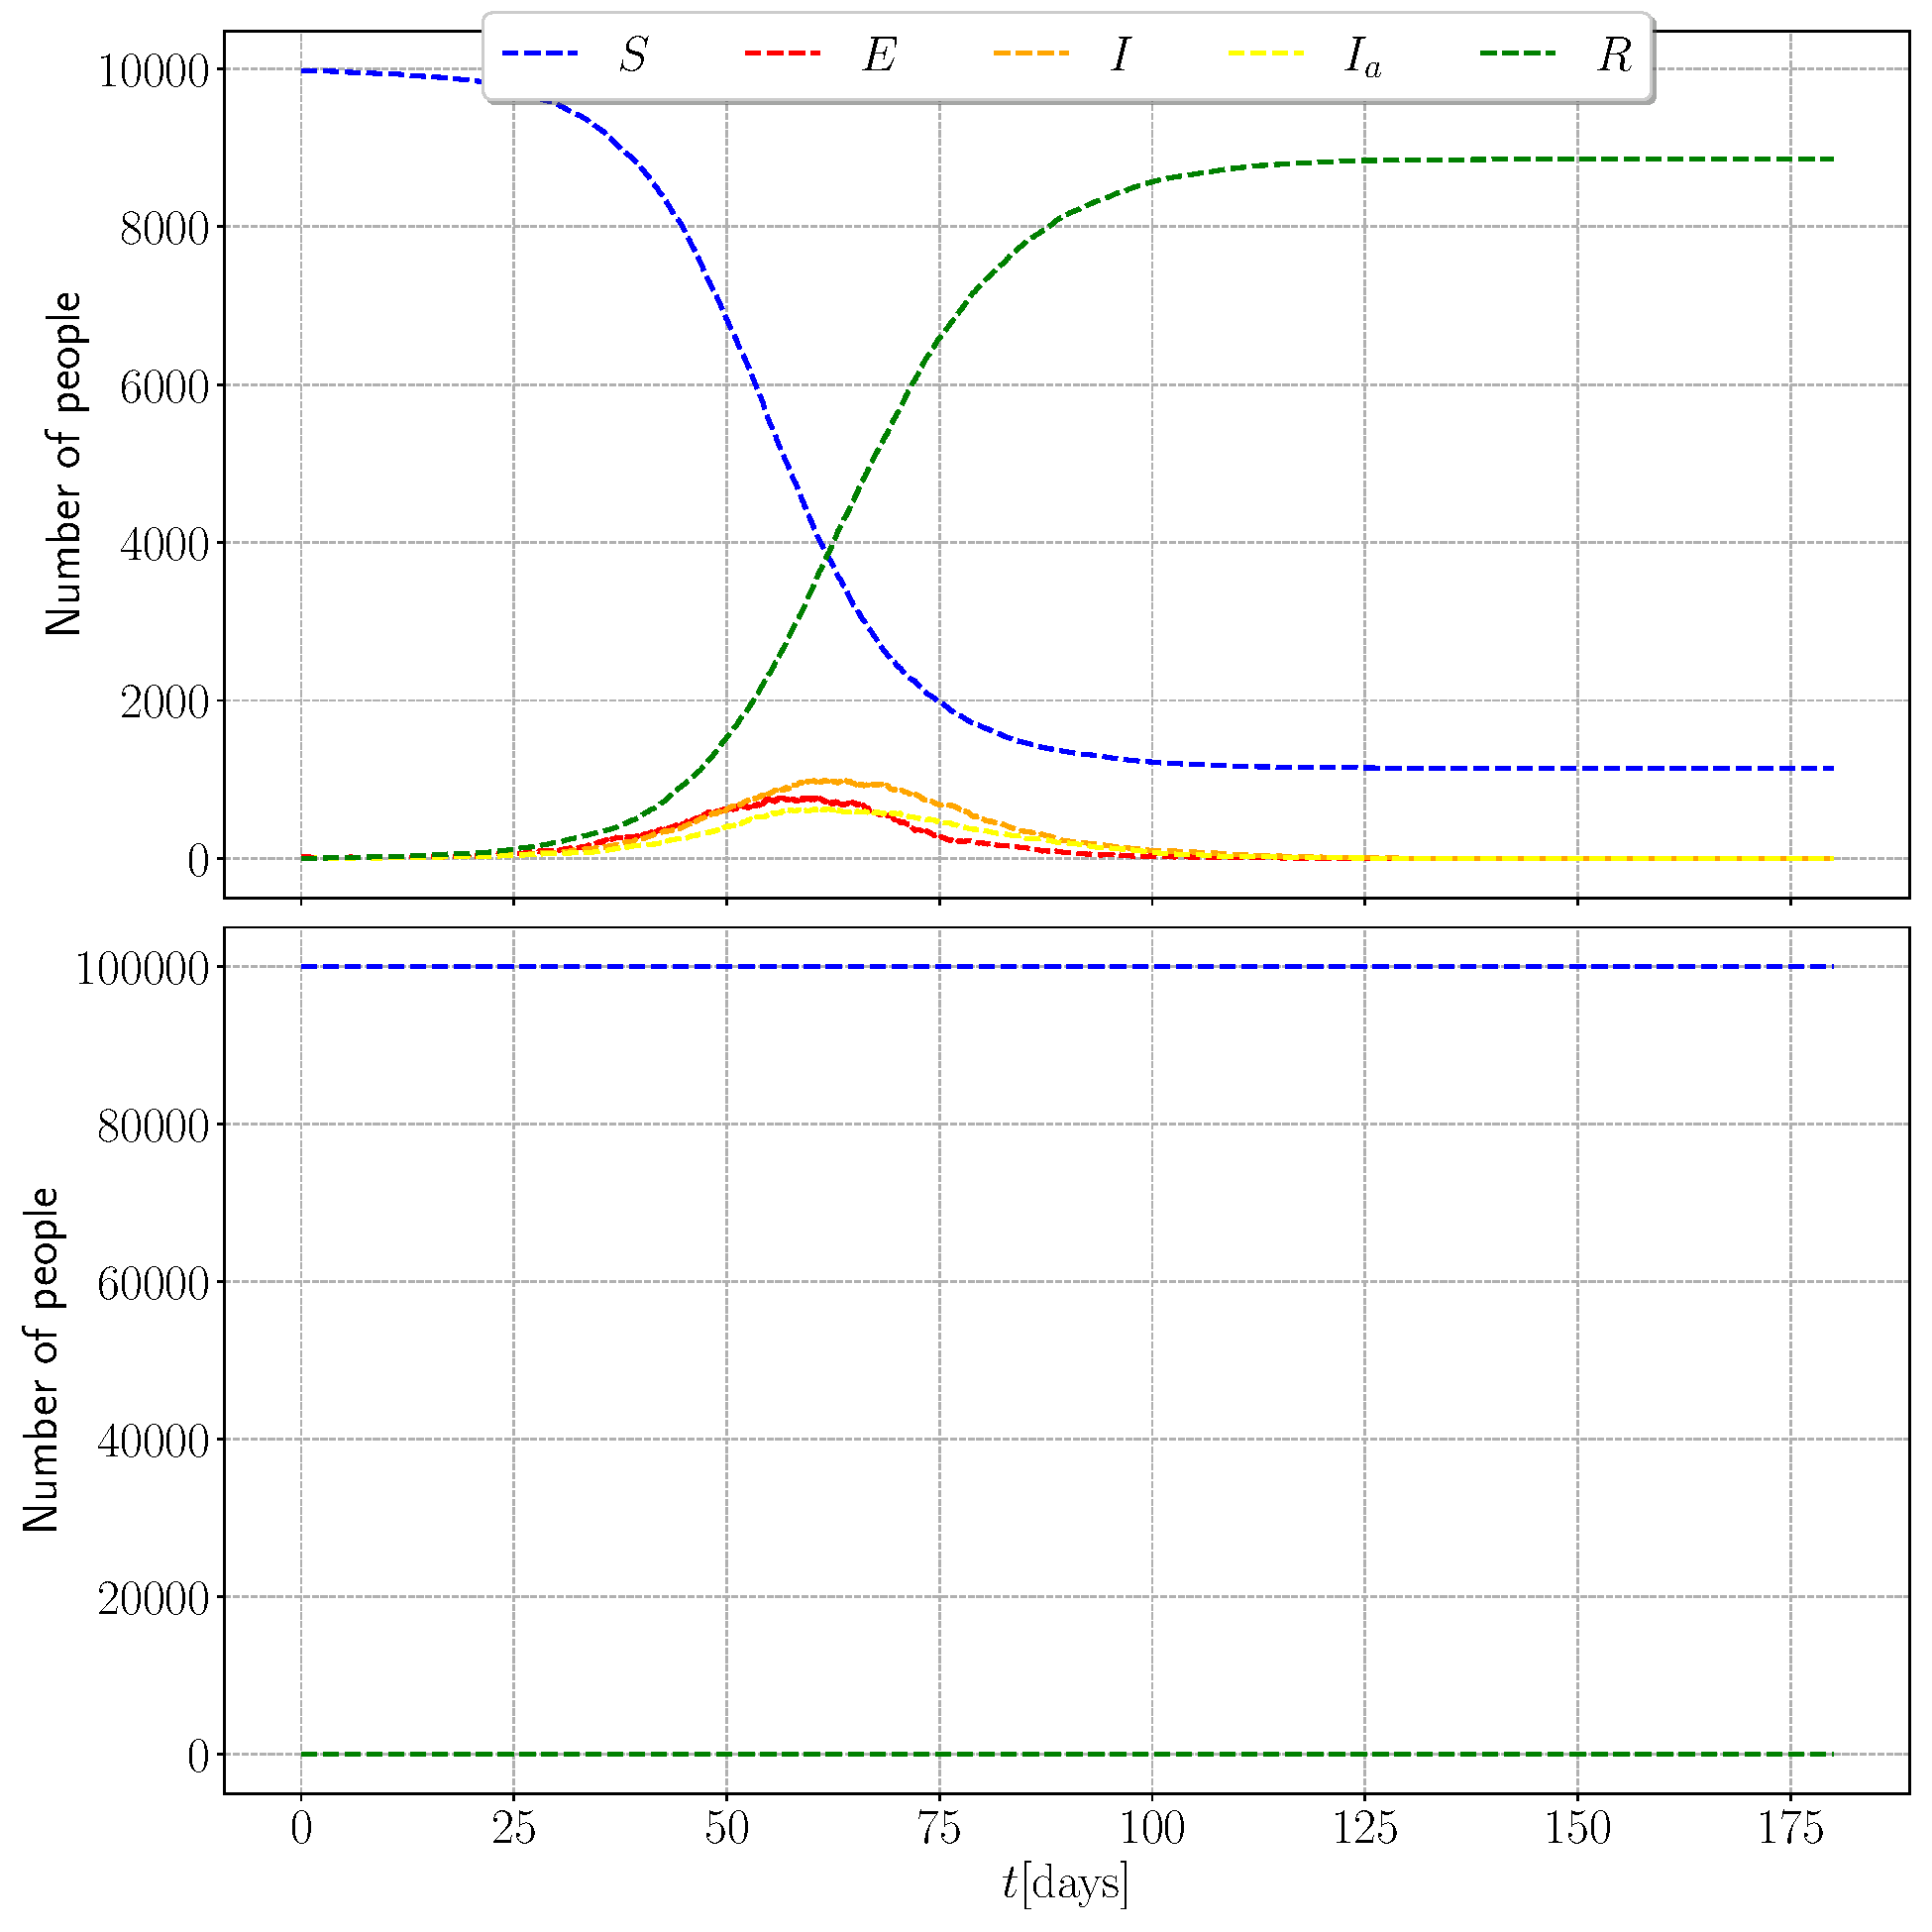
\includegraphics[width=0.8\columnwidth]{../fig/test_commuter.pdf}
	\caption{Solutions of Stochastic SEIIaR commuter model for the $2$-city case, with the matrix $\mathbf{\widetilde{M}}$ in equation \eqref{eq:test_matrix}.}
	\label{fig:test_commuter}
\end{figure}

\clearpage
\section{Problem 2D: Larger stochastic SEIIaR Commuter model}

\subsection{a) 10 city simulation}

We use the framework developed in the previous section to simulate a larger system of towns, now with $10$ of them. The population matrix for this system is given in equation (11) in the problem sheet \cite{sheet}. We initialise the system with all people susceptible, except for $25$ exposed in town $2$. The time evolution of $10$ realisations of the different states is shown in figure \ref{fig:commuter_10city}. 

\begin{figure}[htb]
	\centering
	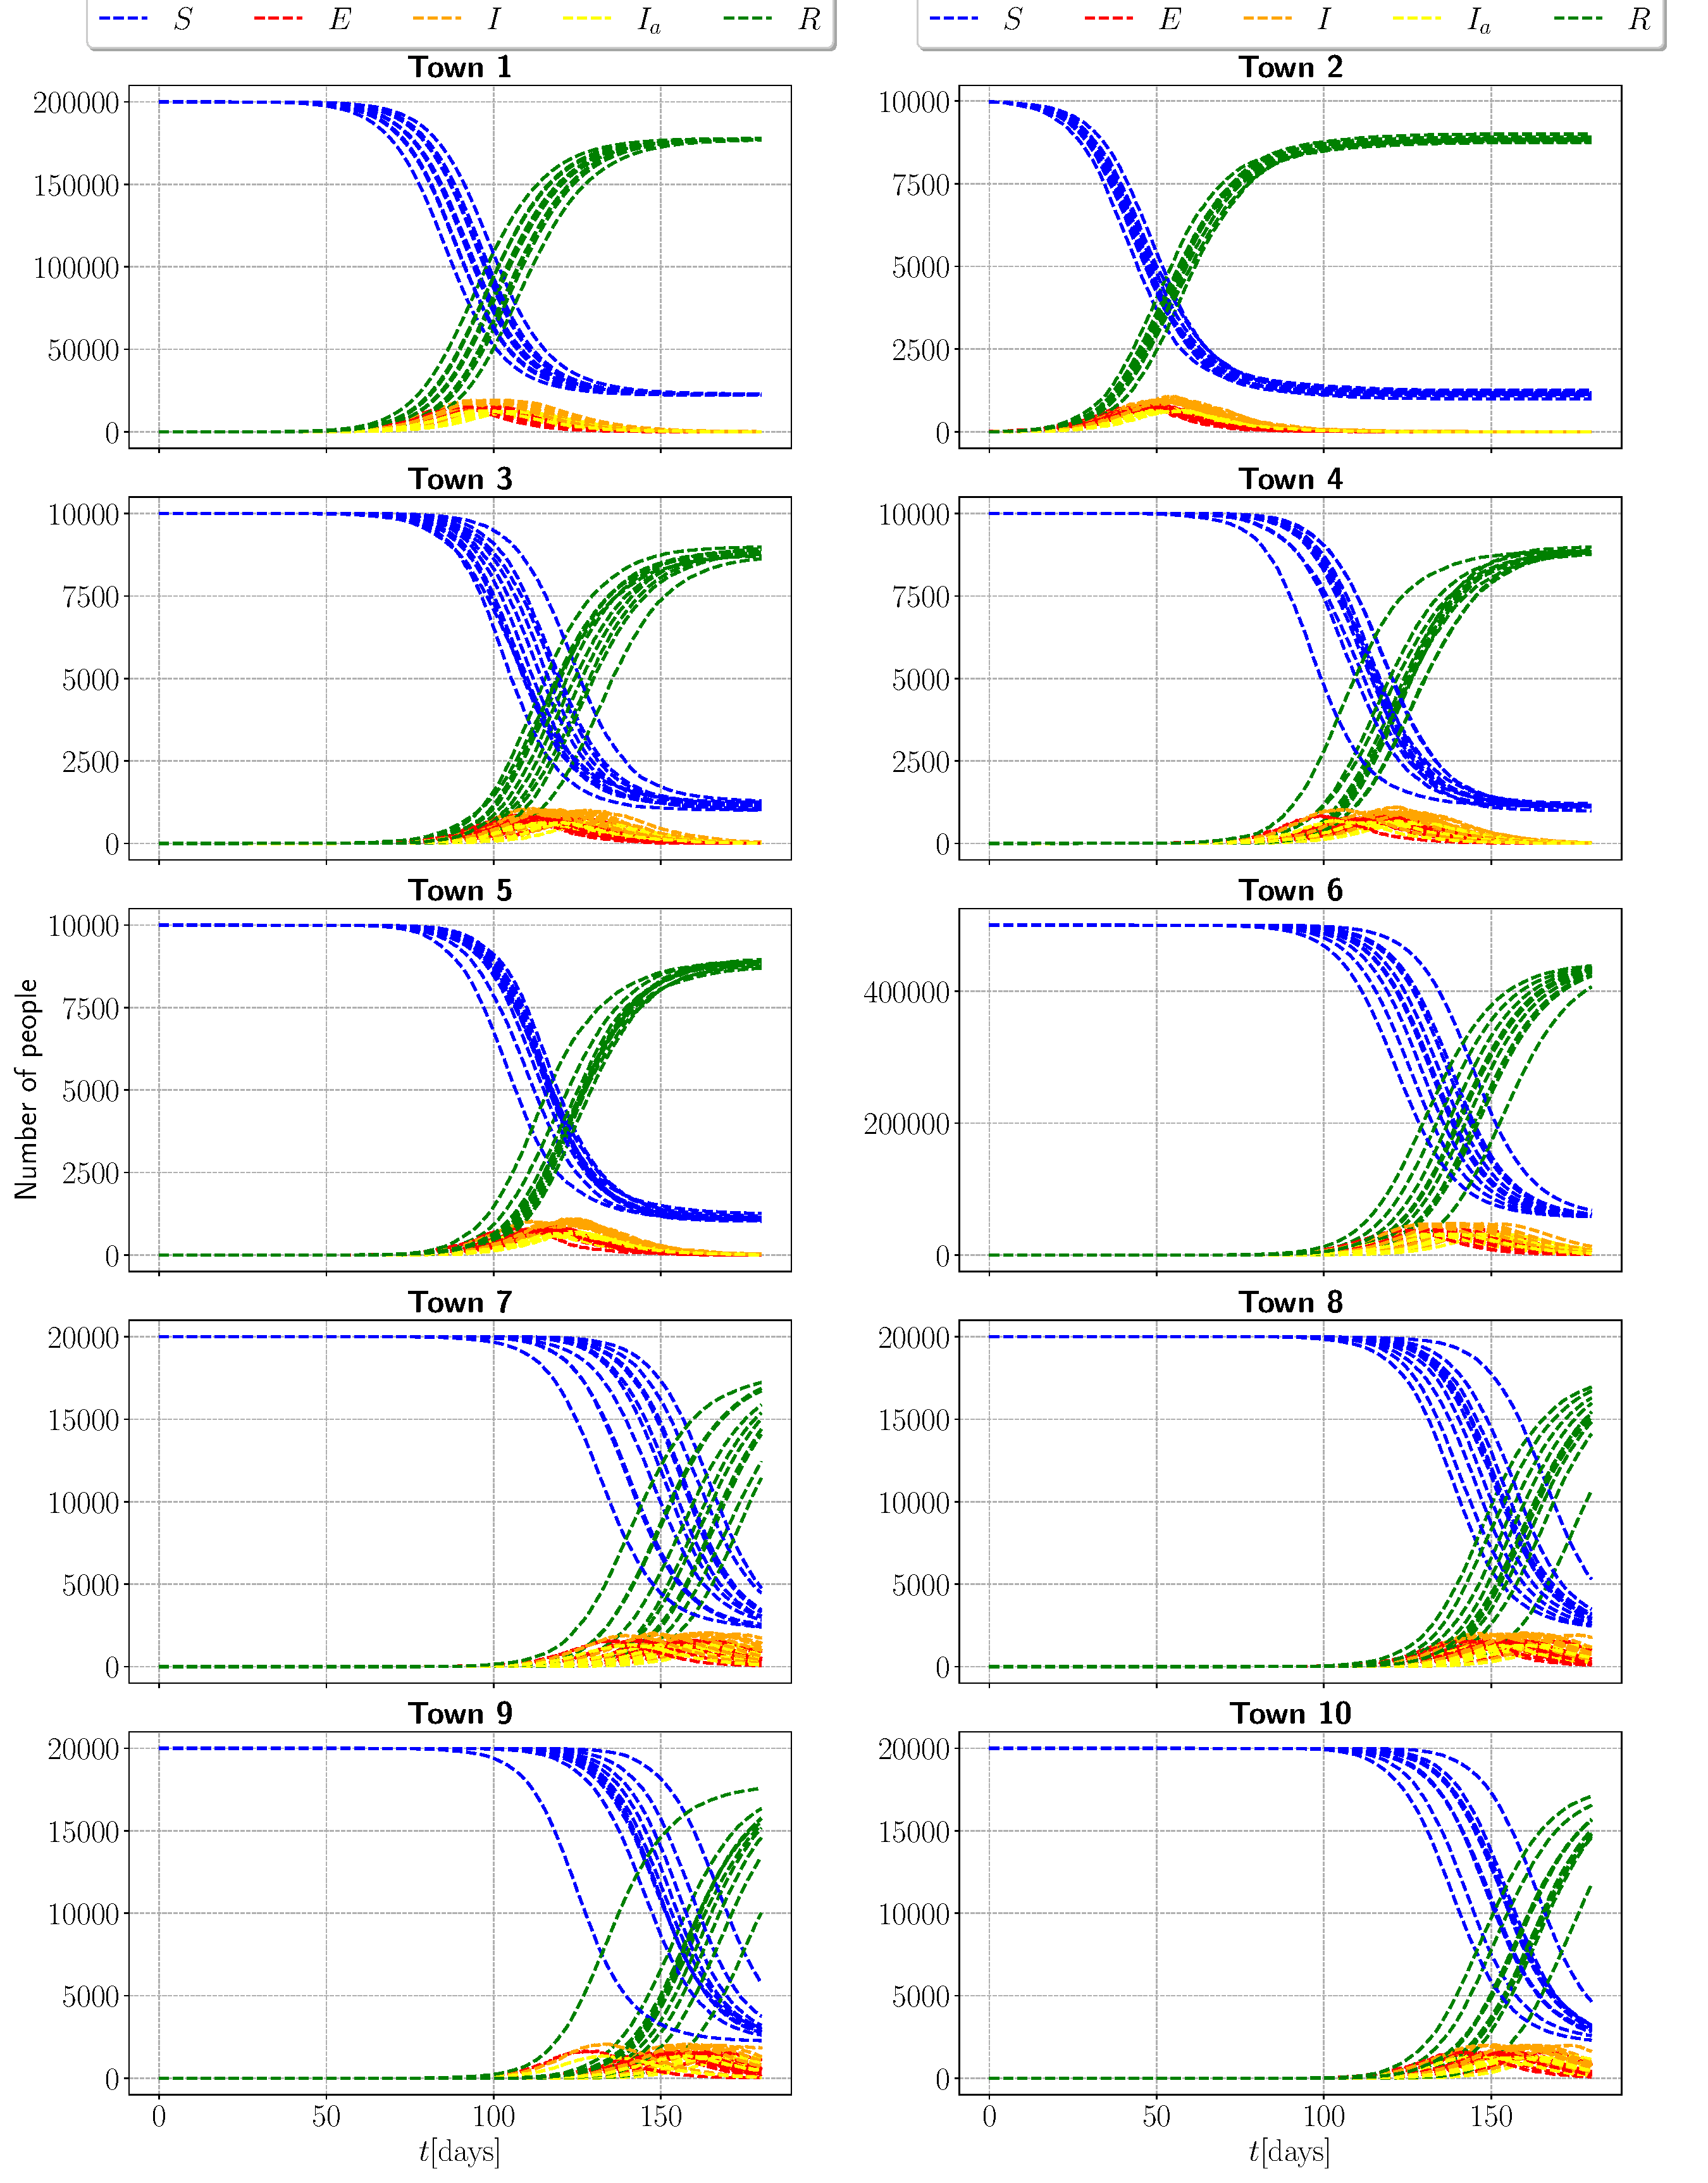
\includegraphics[width=0.87\columnwidth]{../fig/2Ea_commuter.pdf}
	\caption{Solutions of Stochastic SEIIaR commuter model for the $10$-city scenario.}
	\label{fig:commuter_10city}
\end{figure}

Figure \ref{fig:commuter_10city} clearly shows that the epidemic evolves fastest in town $2$, where it began. This is as expected. Furthermore, we see that the second fastest evolution is in town $1$, which is the closest connection to town $2$ in the sense that the commuters of town $2$ only travels to town $1$. This is also a reassuring fact, indicating a correct implementation. Interestingly, for the towns with less connections to town $2$ --- e.g. town $9$ and $10$ --- we see that the evolution lags approximately $100$ days behind, and there seems to be a wider spread between each of the $10$ realisations. The increasing spread may be explained by the fact that small delays in each realisation in the beginning become exceedingly large for another town, as some time must naturally pass for the infections to be exported here.

\subsection{b) $356$ city simulation}

In this problem we use the full population structure handed out along with the problem set. We are here only interested in the number of municipalities with more than $10$ infected people as a function of time ($\eqqcolon \mathcal{N}(t)$), so we modify the commuter solver described in algorithm \ref{alg:commuter} to only keep the current and previous state of the system at each time step, and to calculate $\mathcal{N}$ for each time step, as described in the code overview section. 

\begin{figure}[htb]
	\centering
	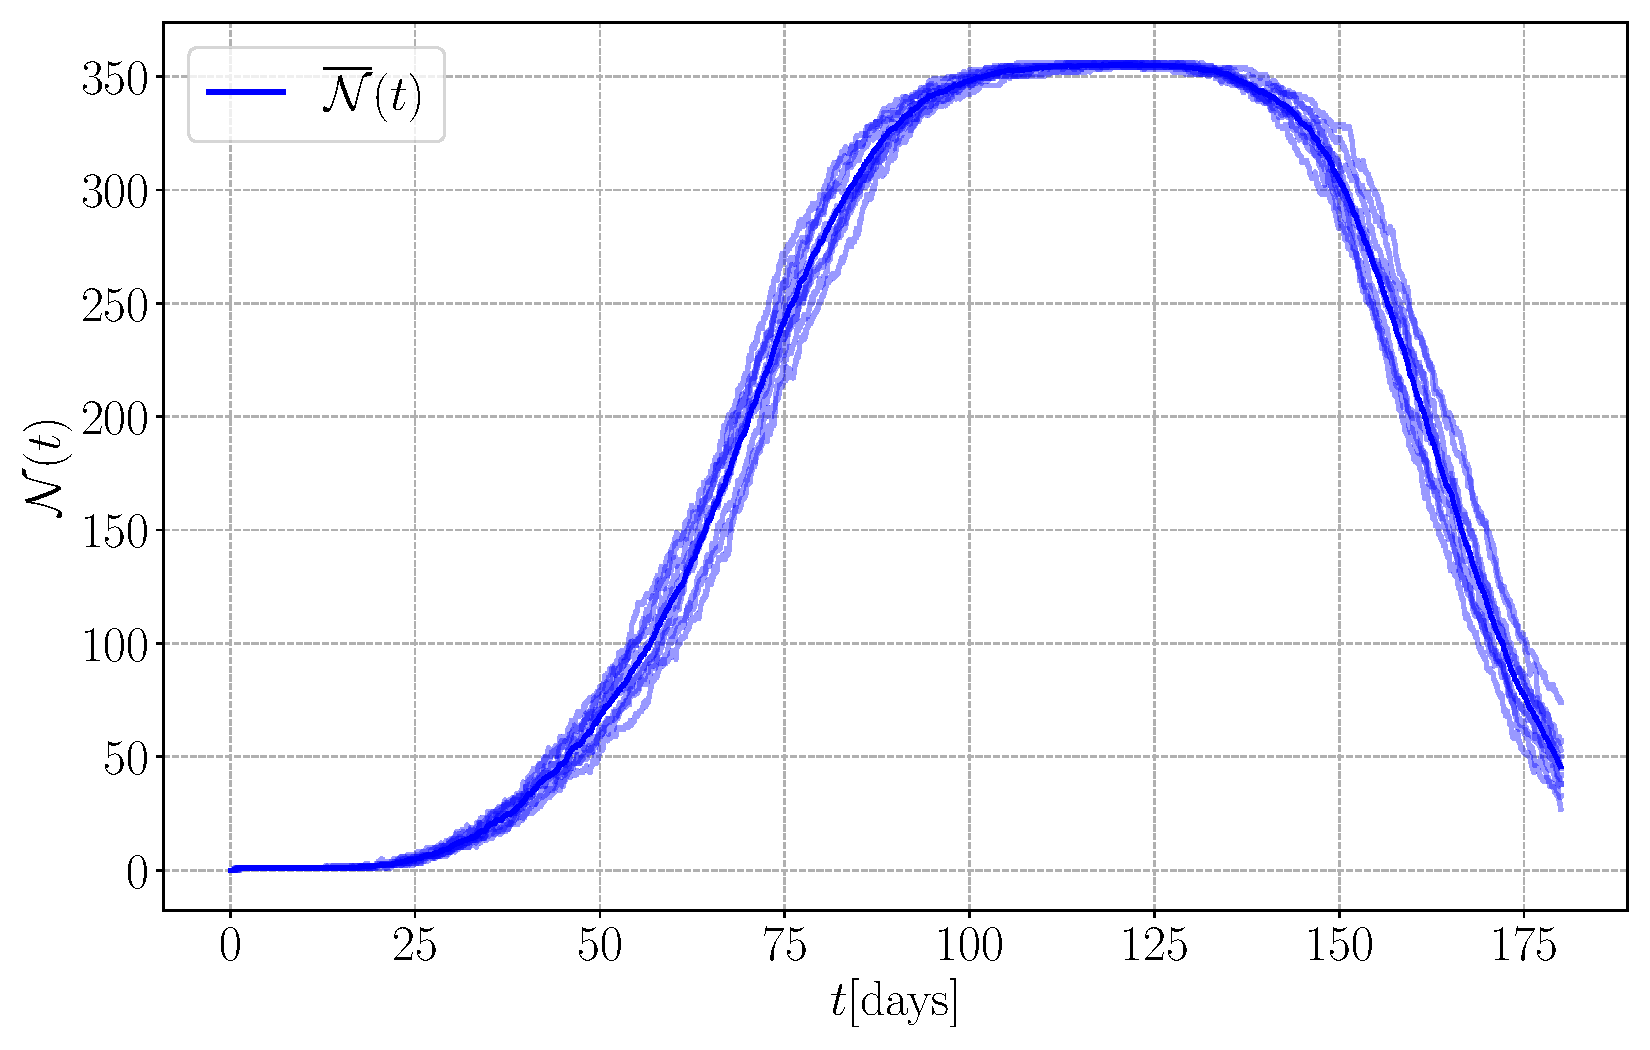
\includegraphics[width=0.9\columnwidth]{../fig/2Eb_N.pdf}
	\caption{Number of municipalities with more than $10$ infected people a a function of time. The mean is shown in the thick black line, while the $10$ realisations are shown in opaque blue lines.}
	\label{fig:infected_Eb}
\end{figure}

We initialise the system with $50$ exposed people in municipality $1$, and the rest being susceptible, and simulate for $180$ days with the parameters specified in the problem sheet \cite{sheet}. $\mathcal{N}(t)$ for 10 realisations of this simulation is shown in figure \ref{fig:infected_Eb}. This figure shows that the infections have spread to all of the municipalities after roughly $110$ days, and that a significant amount of people start to recover after $150$ days. Only about $50$ municipalities have more than $10$ infected individuals when $180$ days has passed, on average.    

\subsection{c) Reduced number of commuters in $356$ city simulation}

To study the effect of making more people work from home, we change the population matrix by dividing the off-diagonal elements by $10$, rounding to the nearest integer, and adding the remaining number of people to the diagonal. We show visually the difference between these two population matrices in figure \ref{fig:matrices}.  
\begin{figure}[htb]
	\centering
	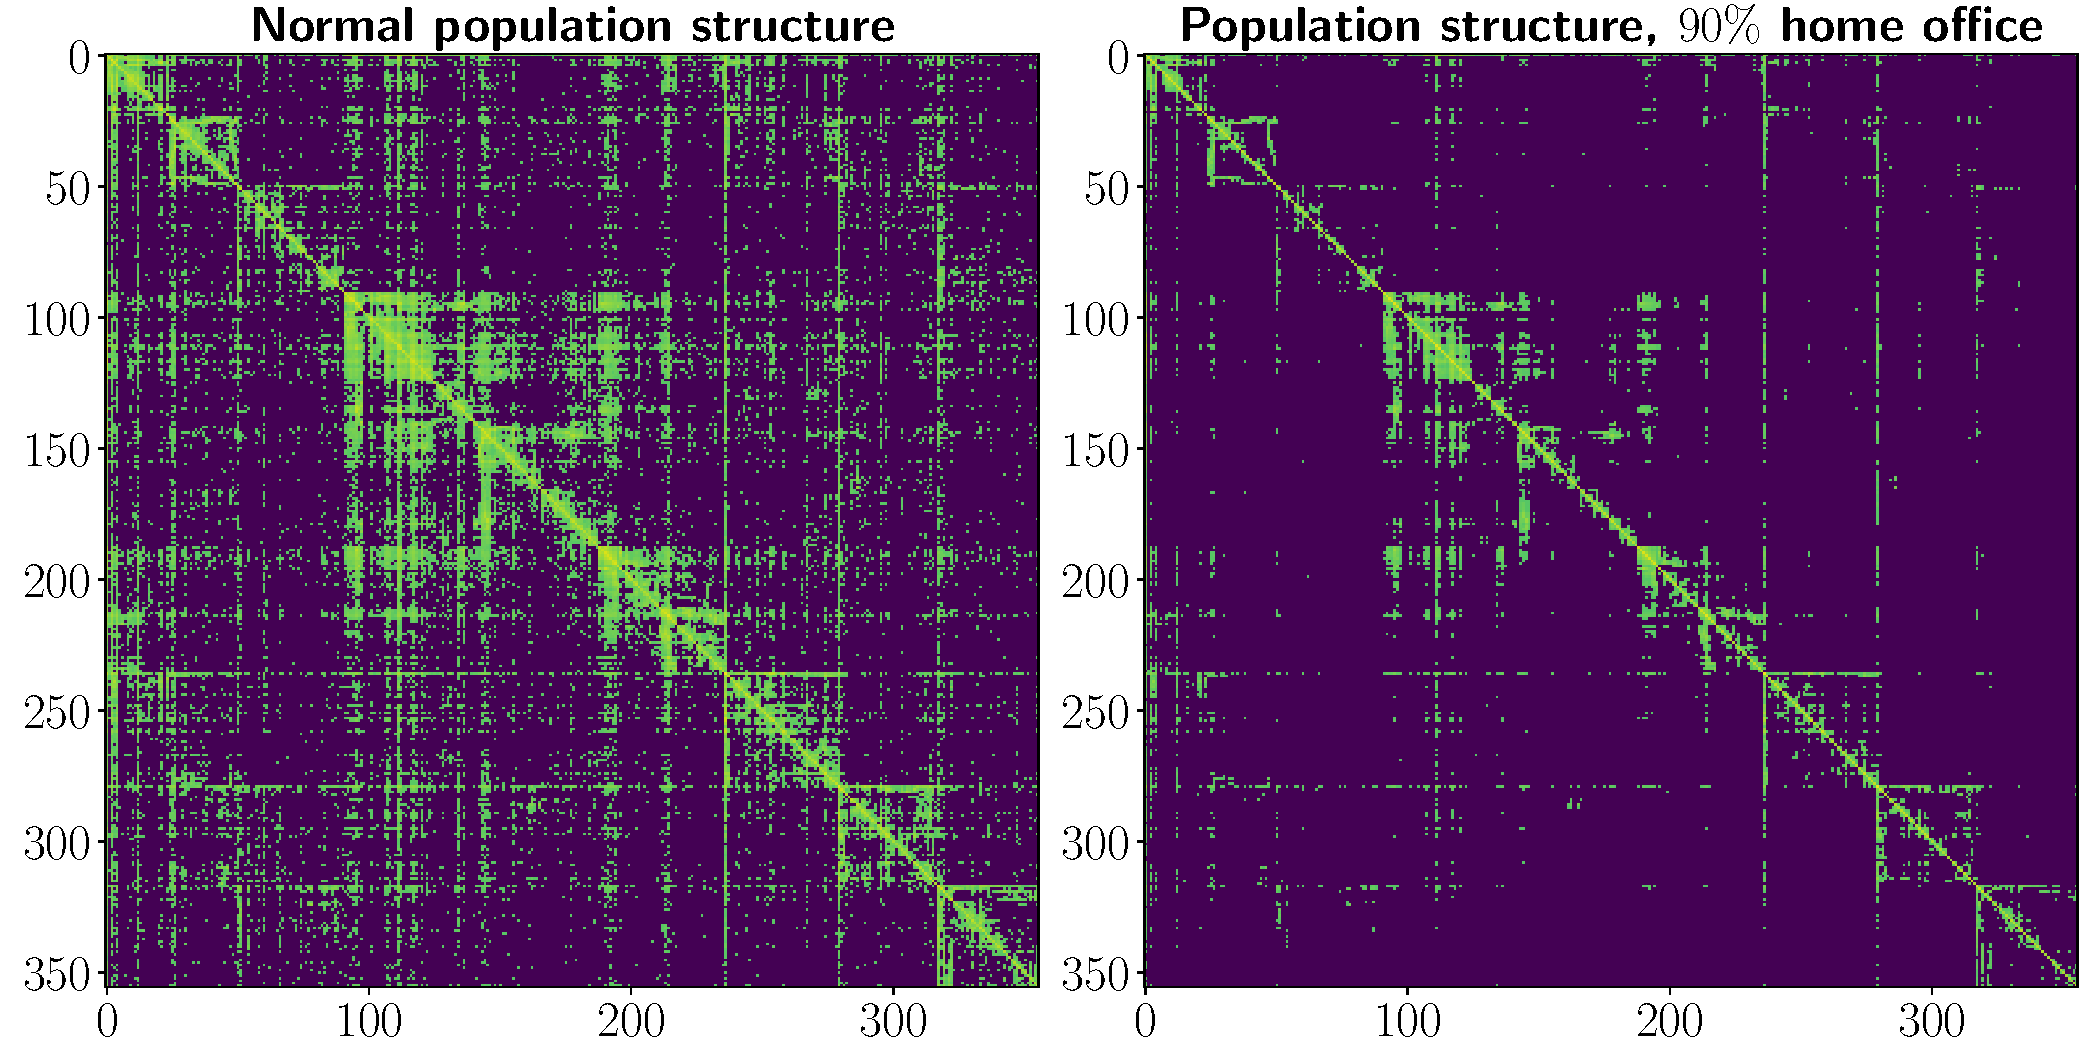
\includegraphics[width=0.9\columnwidth]{../fig/matrices.pdf}
	\caption{Population structures used for problem 2Eb and 2Ec respectively. The purple values are 0, and the numbers values of the entries are logarithmically scaled.}
	\label{fig:matrices}
\end{figure}
\begin{figure}[h!]
	\centering
	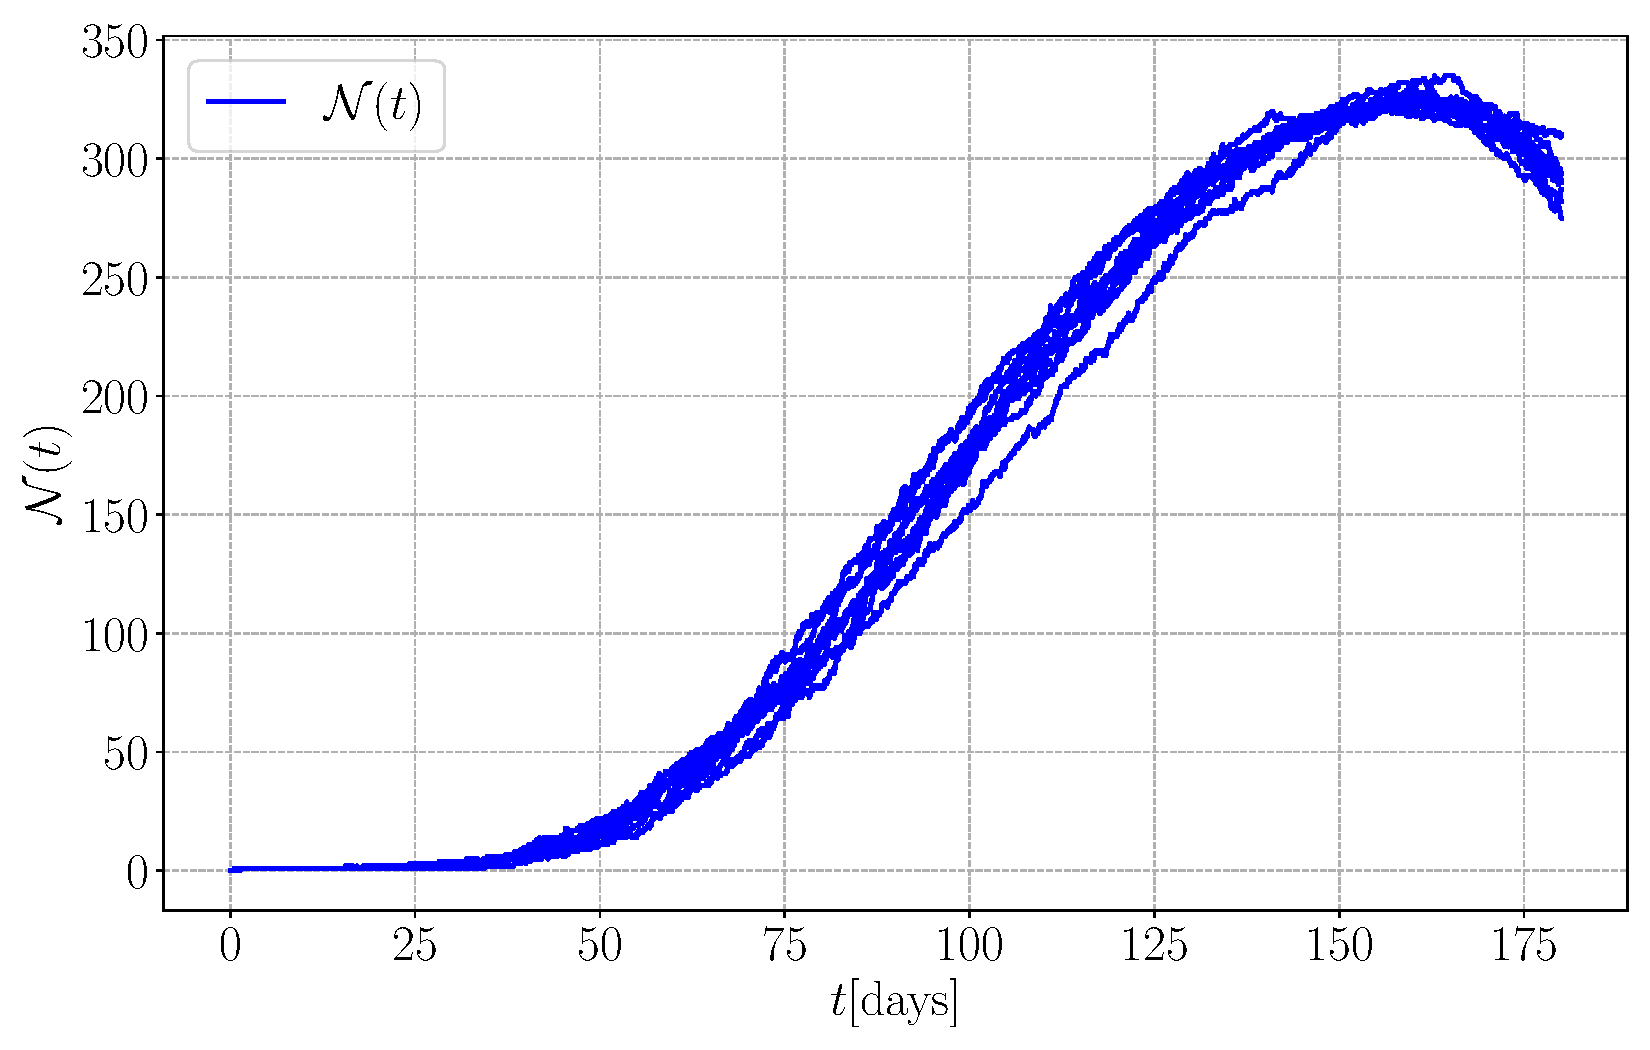
\includegraphics[width=0.9\columnwidth]{../fig/2Ec_N.pdf}
	\caption{Number of municipalities with more than $10$ infected people a a function of time, with reduced travelling.  The mean is shown in the thick black line, while the $10$ realisations are shown in opaque blue lines.}
	\label{fig:infected_Ec}
\end{figure}

We run the same simulation as above, and display the number municipalities with more than $10$ infected people as a function of time, $\mathcal{N}(t)$,  in figure \ref{fig:infected_Ec}. Clearly, the effect of reduced travelling is to reduce the rate of infection spread. In figure \ref{fig:infected_Eb} we see that $\mathcal{N}$ saturates after about $110$ days, while in figure \ref{fig:infected_Ec} it never even reaches the case where $\mathcal{N}$ is $356$. The increase in $\mathcal{N}(t)$ is seen to be much slower in this case, and the peak of the curve occurs after roughly $150$ days. As $\mathcal{N}(t)$ essentially is a measure of the degree of spread in the infections, we see that the effect of reducing travelling between municipalities reduces the geometric spread of the infections, exactly as we would intuitively expect. A side effect of reducing the spatial spreading of the infections is however to increase its spread in time. This is clearly seen by the fact that there are still over $200$ municipalities with more than 10 infected people left after $180$ days in the case of $90 \, \%$ home office. 



%\newpage
%\part{Conclusion}
%\input{./conc}

\bibliographystyle{alpha}
\bibliography{references}

\end{document}